\documentclass[
  11pt,					% Schriftgröße
  DIV=13,				% Seitenlayout (Satzspiegel)
  parskip=quarter,		% Abstand zwischen Absätzen
  oneside,				% Einseitig
%  headsepline,
  headings,	
%  draft,				% Korrekturfassung
  ]{scrreprt}			% scrartcl	


\usepackage[utf8]{inputenc}
\usepackage[ngerman,english]{babel}
\selectlanguage{english}

\usepackage{graphicx}
\usepackage{float}
\graphicspath{{bilder/}}
\usepackage{svg}
\usepackage{listings}
\usepackage{verbatim}
\usepackage{lmodern}
\definecolor{codegreen}{rgb}{0,0.6,0}
\definecolor{codegray}{rgb}{0.5,0.5,0.5}
\definecolor{codepurple}{rgb}{0.58,0,0.82}
\definecolor{backcolour}{rgb}{0.95,0.95,0.92}


\lstdefinestyle{mystyle}{
	backgroundcolor=\color{backcolour},   
	commentstyle=\color{codegreen},
	keywordstyle=\color{magenta},
	numberstyle=\tiny\color{codegray},
	stringstyle=\color{codepurple},
	basicstyle=\ttfamily\footnotesize,
	breakatwhitespace=false,         
	breaklines=true,                 
	captionpos=b,                    
	keepspaces=true,                 
	numbers=left,                    
	numbersep=5pt,                  
	showspaces=false,                
	showstringspaces=false,
	showtabs=false,                  
	tabsize=2
}
\lstset{style=mystyle}
\usepackage{ulem}

% Blindtext
\usepackage{blindtext}
 
% Schrifteinstellungen
\usepackage{lmodern} 		% Vektorschrift
\renewcommand{\familydefault}{\sfdefault}
\usepackage{sansmath}
\sansmath 
\usepackage{microtype}

% Literatur einbinden
\usepackage{csquotes}	% Steuerung der Anführungszeichen
\usepackage[
  backend=bibtex,		% Sortier-Compiler
  style=numeric-comp,	% Zitationsstil
  ]{biblatex}

% Mathemodus
\usepackage{amsmath,amssymb}

% Trennung
\hyphenation{Crash-zo-ne}                    
\addbibresource{ref/ref.bib} %Citavi Reference Datei

% Kopf- und Fußzeile
\usepackage[
headsepline,	% Kopfzeilen-Sepparationslinie
automark,		% Lebende Kolumnentitel
]
{scrlayer-scrpage}
\pagestyle{scrheadings}		

\ohead*{\headmark}

\usepackage{abstract}
\usepackage{adjustbox}
\usepackage{tabularx}

%%%%%%%%%%%%%%%%%%%%%%%%%%%%%%%%%%%%%%%%%%%%%%%%%
%%%%%%%%%%%%%%%%%%%%%%%%%%%%%%%%%%%%%%%%%%%%%%%%%
%%%%%%%%%%%%%%%%%%%%%%%%%%%%%%%%%%%%%%%%%%%%%%%%%
%%%%%%%%%%%%%%%%%%%%%%%%%%%%%%%%%%%%%%%%%%%%%%%%%
%%%%%%%%%%%%%%%%%%%%%%%%%%%%%%%%%%%%%%%%%%%%%%%%%
%%%%%%%%%%%%%%%%%%%%%%%%%%%%%%%%%%%%%%%%%%%%%%%%%
%%%%%%%%%%%%%%%%%%%%%%%%%%%%%%%%%%%%%%%%%%%%%%%%%
%%%%%%%%%%%%%%%%%%%%%%%%%%%%%%%%%%%%%%%%%%%%%%%%%



% Titelseite
\titlehead{
  \begin{center}
  	
\includegraphics[width=0.5\textwidth]{thi_logo_cropped}
  \end{center}
}

\title{Development of a mobile application for the algorithmic attribution of symptoms to potential diseases}

\subtitle{ \vspace{2ex} \LARGE BACHELOR THESIS}

\author{Angelina Petzold\\Immatriculation Number: 00108359}

\date{}

\publishers{
  \begin{tabular}{rl}
   \textbf{First Examiner} 		& Prof. Dr. Sebastian Apel 	\\
   \textbf{Second Examiner} 	& Prof. Dr. Marc Aubreville \\
   \textbf{Start Date} 			& October 11, 2022 		\\
   \textbf{Submission Date} 	& March 11, 2023		\\
  \end{tabular}
  }
  
% Rückseite der Titelseite
\uppertitleback{\begin{center}
		Development of a mobile application for the algorithmic attribution of symptoms to potential diseases
\end{center}}

\lowertitleback{\begin{center}
Technische Hochschule Ingolstadt
	\end{center}}



\newcommand\frontmatter{%
	\cleardoublepage
	%\@mainmatterfalse
	\pagenumbering{roman}}

\newcommand\mainmatter{%
	\cleardoublepage
	% \@mainmattertrue
	\pagenumbering{arabic}}

\begin{document}
  
  \maketitle
  
  \frontmatter
  
  
%% ABSTRACT %%

\selectlanguage{english}
{
	\raggedbottom
	\centering
	\vspace{0.9cm}
	\large
	\textbf{ABSTRACT}
	
	\adjustbox{minipage=0.8\textwidth}{
		\vspace{1.5cm} 
		  
	\par}
 	\pagebreak

	\selectlanguage{ngerman}
	\vspace{0.9cm}
	\large
	\textbf{PREAMBLE}
	
	\adjustbox{minipage=0.8\textwidth}{
		\vspace{1.5cm} 
		   
	\par}
	\pagebreak

	\selectlanguage{ngerman}
	\vspace{0.9cm}
	\large
	
	\textbf{\centering ACKNOWLEDGEMENTS}
	\vspace*{\fill}

	Mein hauptsächlicher Dank gilt meinem Betreuer Professor Doktor Sebastion Apel für seine hilfreichen Anregungen während des gesamten Betreuungszeitraumes. Die Freiheit, die er mir bei der Wahl des Themas gelassen hat, war nicht selbstverständlich.
	\newline \\
	Auch die Teilnehmerinnen und Teilnehmer meiner Befragung haben durch ihre Auskunftbereitschaft und interessanten Beiträge meine Bachelorarbeit wesentlich mitgeprägt.
	\newline \\
	Letztlich richte ich auch ein Dankeschön an meine Kommilitonin  Frau Jenny Hofbauer für das ausführliche Korrekturlesen und dem Mut machen während der gesamten Arbeit.
	
	\vspace{1cm}
	\noindent\hfil\rule{0.5\textwidth}{.4pt}\hfil
	\vspace{1cm}
	
	My main thanks go to my supervisor Professor Doctor Sebastion Apel for his helpful suggestions during the whole period of supervision. The freedom he gave me in choosing the topic was not self-evident.
	\newline \\
	The participants in my survey also played a major role in shaping my bachelor thesis through their willingness to provide information and interesting contributions.
	\newline \\
	Finally, I would also like to thank my fellow student Ms. Jenny Hofbauer for her detailed proofreading and encouragement throughout the thesis.
	\vspace*{\fill}
	\pagebreak


\par}
  
  \tableofcontents
  
  \mainmatter
  
  
%% INTRODUCTION %% 
\chapter{Introduction}

% PROBLEM
\section{The Bachelor's Thesis Problem}
People in Germany are becoming more interested in physical and mental health matters. This is most likely attributed to the COVID-19 pandemic that has been circulating in recent years \cite{.bahn-bonn}. Along with positive outcomes, such as increased care for fellow citizens and greater awareness of health issues, the consistent growth of interest in health issues is causing problems. With an increasing number of anxious and concerned patients, medical practices and general practitioners have long since exceeded their capacity limits and have reached their breaking point \cite{.sok}. Patients also notice this: Overcrowded waiting rooms, long waiting periods, and nerve-racking telephone loops are becoming the norm for doctor visits. The German Medical Association (BAEK) draws attention to a second issue: as society ages, so does the medical industry. Every fifth doctor is about to retire. More than 13\% of doctors are between the ages of 60 and 65, while another 8.5\% are over the age of 65. Over the following few years, this will exacerbate clinics' and offices' already stressful staffing situation \cite{.blatt}. 
\newline \\
The bachelor's thesis problem can be traced back to the preceding situation. The population is fearful, mainly caused by the COVID-19 pandemic, and doctors are reaching their limits. The resulting problems are of great importance. General practitioners are forced to order patient stops and issue access bans \cite{.sok}. This also means that patients needing immediate medical attention may be turned away, and medical care may be denied. In addition to the concerned patients, the number of seriously (COVID-19) ill people has steadily increased. There have been approximately 146,000 deaths in Germany since the start of the pandemic (as of August 19, 2022)\cite{.rki}. As part of this work, a survey was launched to highlight the problem in more detail. The results indicate that around 80\% of those questioned have put off a visit to the doctor in recent years - even though they have suffered from symptoms.
% UMFRAGE ERSTE FRAGE
\begin{figure}[H]
	\centering
	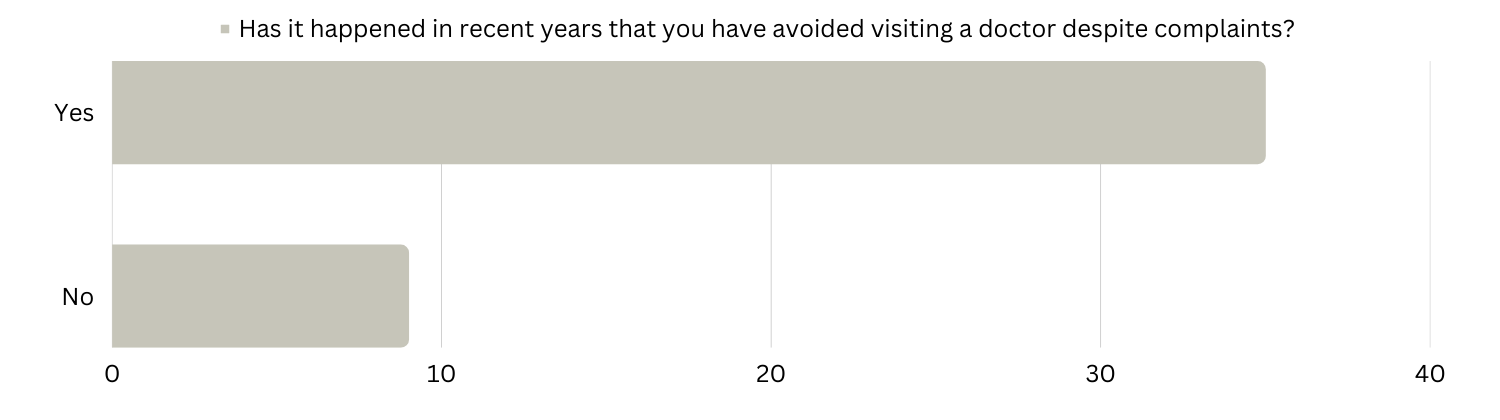
\includegraphics[scale=0.35]{avoidingDoctorYesNo.png}
	\caption[Survey Question]{Survey Question - Avoiding visiting the doctor}
\end{figure}
\noindent 
% UMFRAGE ZWEITE FRAGE
Another question in this survey asked respondents to list the justifications for delaying these doctor visits or the reasons they might consider forgoing a visit to the doctor. Those reasons range from long waiting times to difficulties scheduling an appointment. Figure 1.2 shows the mentioned distribution of the answers. All questions of the survey, together with the answers, can be found in Appendix A.
\begin{figure}[H]
	\centering
	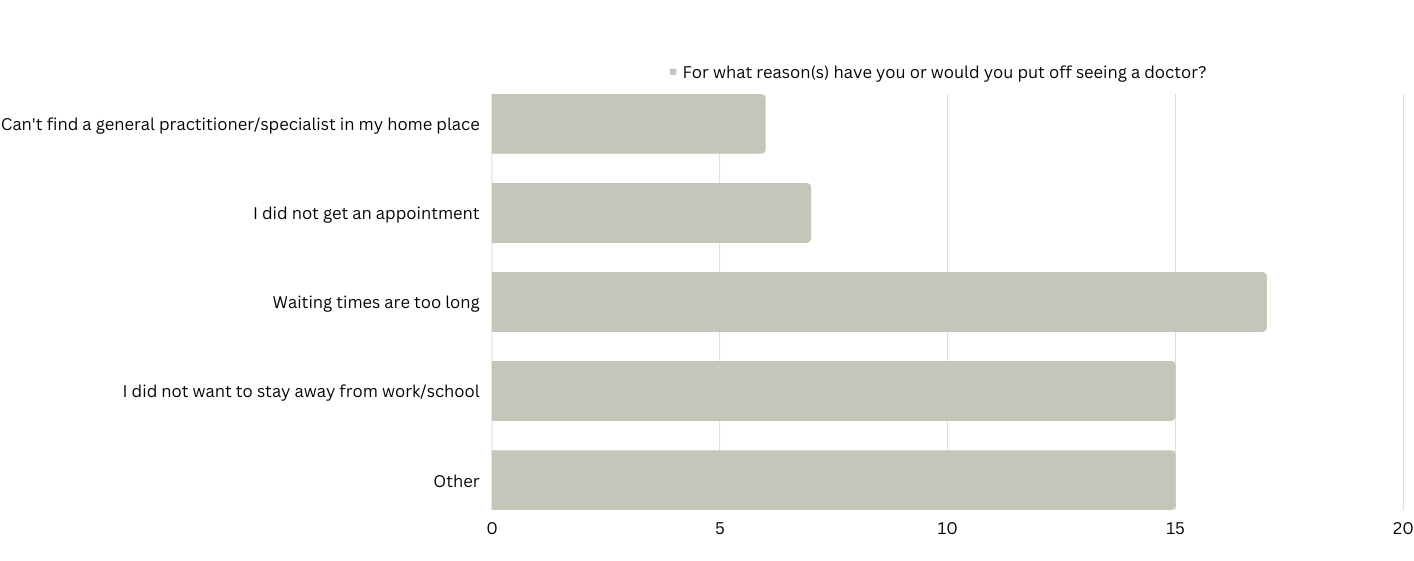
\includegraphics[scale=0.35]{2.png}
	\caption[Survey Question]{Survey Question - Reasons for avoiding to visit the doctor}
\end{figure}
\noindent 

\section{Motivation}
The mentioned problem imposes the question of addressing patients' concerns while relieving the burden on doctors. Digitalization provides a solution to this problem. Online consultation hours and appointment scheduling have recently helped relieve medical practices. Smartphones, in particular, are becoming an increasingly important part of our daily lives. The goal of this bachelor thesis is to provide a method for efficiently minimizing the problems mentioned above through the use of mobile applications. Such an application can advise a worried user and help alleviate their fears.

\section{The Bachelor Thesis Goal}
The goals of the bachelor thesis can be defined as follows:
\begin{itemize}
	\item Requirements analysis for the application
	\item Design and conception of the application
	\item Creation of a database
	\item Comparing different algorithmic disease assignment methods
\end{itemize}
The application should be able to generate a diagnosis based on a user's specified symptoms. This diagnosis is made after successful data gathering regarding the user's symptoms and a subsequent determination of the possible diseases. Another goal of the application is that doctors can expand the database, whereby a verification possibility must be provided to ensure that the person trying to log in is, in fact, a doctor. They should be provided with the possibility to add disease-related data or advice regarding diseases and illnesses for users. In general, this is to create a place for users to get information regarding their health status and, at the same time, get advice on how to improve it. The research question is:
\newline \\
\begin{center}
	\textbf{How can a mobile application for the algorithmic attribution of symptoms to potential diseases be designed and implemented?}
\end{center}

\chapter{Related Works}
This chapter provides an overview of a selection of mobile applications comparable to the one in this work.


\section{Ada} 
\textbf{Ada} is the most popular symptom-detection smartphone application. According to their statements, their users are currently around 12 million, while 28 million symptom analyses have already been completed \cite{.adaHOME}. The application is free in the Play Store and the Apple Store. Disease detection is based on artificial intelligence (AI) developed by medical professionals of the Ada team. Users can provide personal data in their user profile, such as allergies and medication intake. A symptom analysis starts by asking the user what their worst symptom is. Based on the user's answer, the AI searches its medical lexicon for this symptom and asks a symptom-specific question.
An example of this would be to ask the user if he had enough water today for the symptom headache. Ada uses a specially developed reasoning technology to assign symptoms. For this purpose, each symptom and each disease was assigned a joint probability, which makes it possible to calculate the overall probability of the disease for the specific symptom analysis \cite{.adaKI}. After the successful diagnosis, the user can download the diagnosis in portable document format (PDF), while they are also saved internally. The Ada application makes its collection of knowledge available to users in the form of a disease dictionary. Ada also offers an application programming interface (API), which enables healthcare organizations to integrate the AI chatbot into their application with the help of platform-specific SDKs (Software Development Kits)\cite{.adaFAQ} \cite{.adaDOCU}.

\section{Symptom Checker} 
The \textbf{Symptom Checker} is another currently available application. It was created using the programming language C\# and the Unity engine \cite{.symptomchecker}. Here, the user can select from a list of disease specifications. During the survey procedure, a doctor's interview is simulated, where the user is prompted with questions after choosing one of these categories, similar to the Ada application. The most likely condition is then diagnosed based on the patient's responses, and various treatment choices are provided. The application was made specifically for people without medical experience and was created by German doctors and medical experts. According to the developers, an algorithm that accesses a medical database produces the diagnosis \cite{.symptomchecker}. Nothing more can be found about the algorithm and how it works. 

\section{Other Solutions}
In addition to Ada and the Symptom Checker, other applications for symptom detection are available in the Play Store. However, these are less accurate than those mentioned. Some of these applications are only intended as a reference book for symptoms and diseases without a disease determination. In addition to mobile applications, some web applications and websites are available. However, those solutions will not be discussed further in this work since only mobile applications areof interest for this thesis.

\section{Differentiation from other Systems}
In contrast to both of the applications mentioned, the system's knowledge base should be expanded by doctors who are not part of the development team. Similar to the Diagnosis App, the application presented in this work will not request any personally identifiable information from its users. An exception is a case when users wish to identify themselves as doctors. Unlike Ada, the diagnoses are not generated using AI but are calculated by an algorithm. As already mentioned, the calculation process of the Diagnosis App cannot be determined, and therefore no differentiation can be made from this application. With a realistic view, this application cannot work as accurately as AI, which has been trained since 2011. This work should not replace Ada as the market leader, nor the Diagnosis App, but describe the possible conception and implementation of such an application while comparing different calculation possibilities of the diseases based on the user symptoms.





  
  

%% EINLEITUNG %% 
\chapter{Fundamentals}
This section explains basics needed to understand the rest of the work. Since the Flutter framework and the Dart programming language with which this application is to be developed are not topics that are dealt with in a computer science degree, they will also be discussed.
\section{Flutter and Dart}
The framework used to develop the disease-detection application will be Flutter, which is an open-source-UI-Kit developed by Google. Flutter uses the open-source programming language Dart, which at first was designed for building Google Chrome browser-applications and later on benefited greatly from various improvements since it was released back in 2011. The programming language consequently evolved from having a lot in common with JavaScript to sharing many features with C\# and Java. The Flutter and Dart ecosystem, which is brimming with open-source packages created by other developers from around the world, is one of the framework's best features. It enables programmers to create visually stunning applications in the shortest amount of time, by including packages from developers all over the world. Also, Dart is a client-optimized gneral-purpose programming language that supports cross-platform development. This implies that this application will be created with a single code base yet will run on both Android- and iOS-smartphones. Furthermore, the program may be launched as a web application and utilized on embedded devices. However, as part of the bachelor thesis, the development and testing process will be entirely focused on Android development. Dart is also a statically-typed language, which means that the type of each variable must be explicitly declared, making it easier to catch bugs and other issues early on in the development process. With null safety, Dart ensures that variables cannot be assigned a null value unless they are explicitly declared as nullable. This means that if a variable is expected to have a non-null value, it must be initialized with a non-null value, and any attempts to assign a null value to it will result in a compile-time error. This helps prevent null reference errors and makes it easier to write code that is safe and predictable. [QUELLE:DART/OVERVIEW]

\subsection{Flutter: Everything is a Widget}
When researching how Flutter functions, it's common to come across the phrase "In Flutter, everything is a widget." The difference between Flutter's widgets and those in other Frameworks' components is that Flutter's widgets can specify how the application's user interface should appear. Eric Windmill was able to divide the widgets into various groups in his book Flutter in Action [flutter in action, s 58]:

\begin{itemize}
	\item \textbf{Layout:} 
	Widgets of this category are able to store children-widgets, an example for such a widget would be a row, column or even a stack.  
	\item \textbf{Structures:} 
	As their name implies, structures aid in organizing the application.
	For instance, MenuDrawer produces a sidedrawer for the application, toasts display a message to the user, and buttons can respond to various click patterns. 
	\item \textbf{Styles:} 
	The developer can style widgets in almost any way using Flutter. With a tool like ButtonStyle, a button's background and foreground colors as well as its shape can all be changed.
	\item \textbf{Animations:} 
	Flutter enables its users to breathe life into their applications with a rich palette of animation options. For instance, Flutter developers can use well-known animation features like curves, which are also used in CSS. 
	\item \textbf{Positioning and Alignment:} 
	Widgets such as Padding and Center allow it to position its child widget. There are also additional widgets, such as Positioned and Alignment, that allow the developer to position elements in a Stack.
\end{itemize}
\noindent 
The categorization created by Eric Windmill provides a decent overview of the possibilities in Flutter. There are undoubtedly a lot more widgets and a lot more usage categories that might be defined. Widgets can be composed, which means nested inside of one another [Flutter in action, s61], so rather than simply returning the widget it describes, a widget's build method really returns a tree of widgets. The DOM in any web browser is comparable to this widget tree. A sample widget returned by a build method is shown in Listing 2.1. Figure 2.1 illustrates the generated widget tree in detail.
\begin{lstlisting}[caption=Flutter Scaffold Example]
	Widget build(BuildContext context) {
		return Scaffold(
		appBar: AppBar(
		title: const Text('Example of the build method'),
		),
		body: const Center(
		child: Text('Hello Reader'),
		),
		);
	}
\end{lstlisting}
\begin{figure}[H]
	\centering
	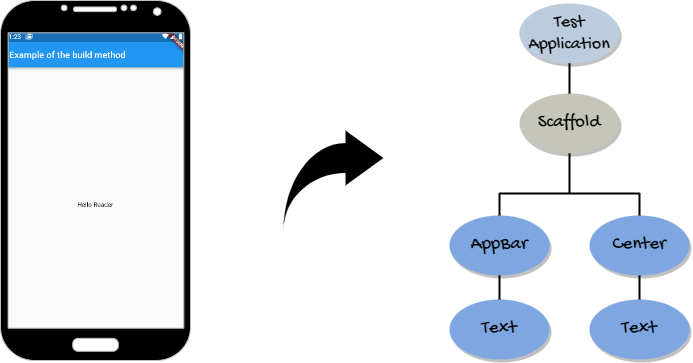
\includegraphics[scale=0.45]{widget_tree.png}
	\caption[Widget Tree of Listing 2.1]{Widget Tree of Listing 2.1}
\end{figure}
\subsection{Flutter: Architectural Layers}
Application architecture refers to how the various components of a mobile or web application are organized and how they interact with each other. A well-designed application architecture helps improve the systems performance, maintainability, scalability but also makes it more modular. [Buch: Software arhcitecture seite 28] Many different application architectural patterns can be used, including layered architecture of which Flutter makes use.  In the context of software development, layered architecture is a common design pattern in which the application is divided into different layers, each layer plays a specific role in the overall functionality of the application. No layer has privileged access to the layers below, and every part of the framework layer is designed to be optional and interchangeable. [Flutter.dev architectural layers] 
\begin{figure}[H]
	\centering
	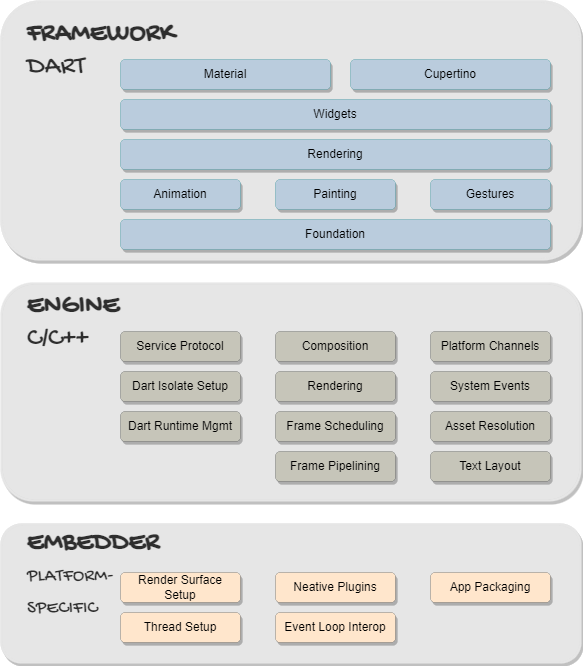
\includegraphics[scale=0.45]{layered_architecture.png}
	\caption[Layered Architecture in Flutter]{Layered Architecture in Flutter[based on Flutter page and TakingFluttertotheWeb page 50/]}
\end{figure}
%\subsection{Darts' Compiler}
%The Dart Compiler parses written code and converts it to machine code. This means that there is no way to directly run written code. [https://www.javatpoint.com/flutter-dart-programming] It's worth mentioning that Dart's compiler technology allows two distinct ways of running written code. Apps built primarily for usage on mobile devices (and desktop devices) can be compiled using the Dart VM, which supports just-in-time compilation (JIT) and ahead-of-time compilation (AOT). The JIT compilation allows the developer, in connection with Flutter, to make use of the hot reload funcionality, which decreases the time comsumption of debugging code. Dart may compile for development or production reasons when it comes to web-based projects. Its web compiler converts Dart to JavaScript. [https://dart.dev/overviewRAUTEplatform]

\subsection{Programming Paradigm}
The programming paradigm of the Dart programming language is object-oriented programming (OOP). This means that it uses objects, classes, and inheritance to organize and structure code. Dart also incorporates some functional programming concepts, such as immutable data and first-class functions, which allow for more concise and elegant code. Additionally, Dart supports asynchronous programming, which enables developers to write code that can run concurrently and handle multiple tasks at the same time. Overall, Dart's combination of OOP and functional programming paradigms makes it a versatile and powerful language for building modern web and mobile applications. The SOLID principles are a set of guidelines for designing object-oriented software. They were introduced by Robert C. Martin in his book "Agile Software Development, Principles, Patterns, and Practices" as a way to improve the maintainability, extensibility, and flexibility of object-oriented code and to develop software that is prone to fewer bugs and has cleaner source code. [https://www.freecodecamp.org/news/solid-principles-explained-in-plain-english/] These principles should be taken into account when developing the application.
\begin{itemize}
	\item \textbf{Single Responsibility Principle (SRP):}
	The single responsibility principle instructs the developer to develop classes and software components in such a way that they take on a maximum of one responsibility. In other words, a class should focus on a single task or piece of functionality, and should not be responsible for multiple unrelated things. This helps to reduce complexity and improve the maintainability, testability, and extensibility of a software system. Another positive side-effect of following this principle is that the written code is easier to understand and error-testing can be done more efficiently.
	
	\item \textbf{Open/Closed Principle (OCP):}
	According to the open-closed principle, software classes should be open for extension but closed for modification, which means a class should be designed in such a way that it can be easily extended or customized without changing its existing code. This allows developers to add new features or behaviors to a class without breaking its existing functionality. This suggests that these classes or software components ought to be developed in a way that allows other system entities to use their essential features without requiring access to the original entity's source code. 
	
	\item \textbf{Liskov Substitution Principle (LSP):}
	The Liskov Substitution Principle (LSP) asserts, in essence, that whenever a function uses a pointer or reference to a base object, it must also use a pointer or reference to any of its derived objects. [Software architecture with c++] One can also say, that it is an extension of the OCP. A subclass should be able to be used wherever its superclass is expected, without breaking the functionality of the program. [stickify, solid design liskov] The Liskov Substitution Principle helps to improve the flexibility and reusability of a software system.
	
	\item \textbf{Interface Segregation Principle (ISP):}
	The Interface Segregation Principle ensures that a clients of a class should not implement an interface that contains methods that are not relevant to its functionality. This helps to avoid creating large and complex interfaces that are difficult to implement and maintain. The Interface Segregation Principle promotes the creation of small, focused, and easy-to-use interfaces. 
	
	\item \textbf{Dependency Inversion Principle (DIP):}
	The key essence of the DIP is that a class should not depend on the specific implementation details of another class. Instead, it should depend on an abstract interface or a set of contracts that define how the two classes should interact.
\end{itemize}

%\begin{figure}[H]
%	\centering
%	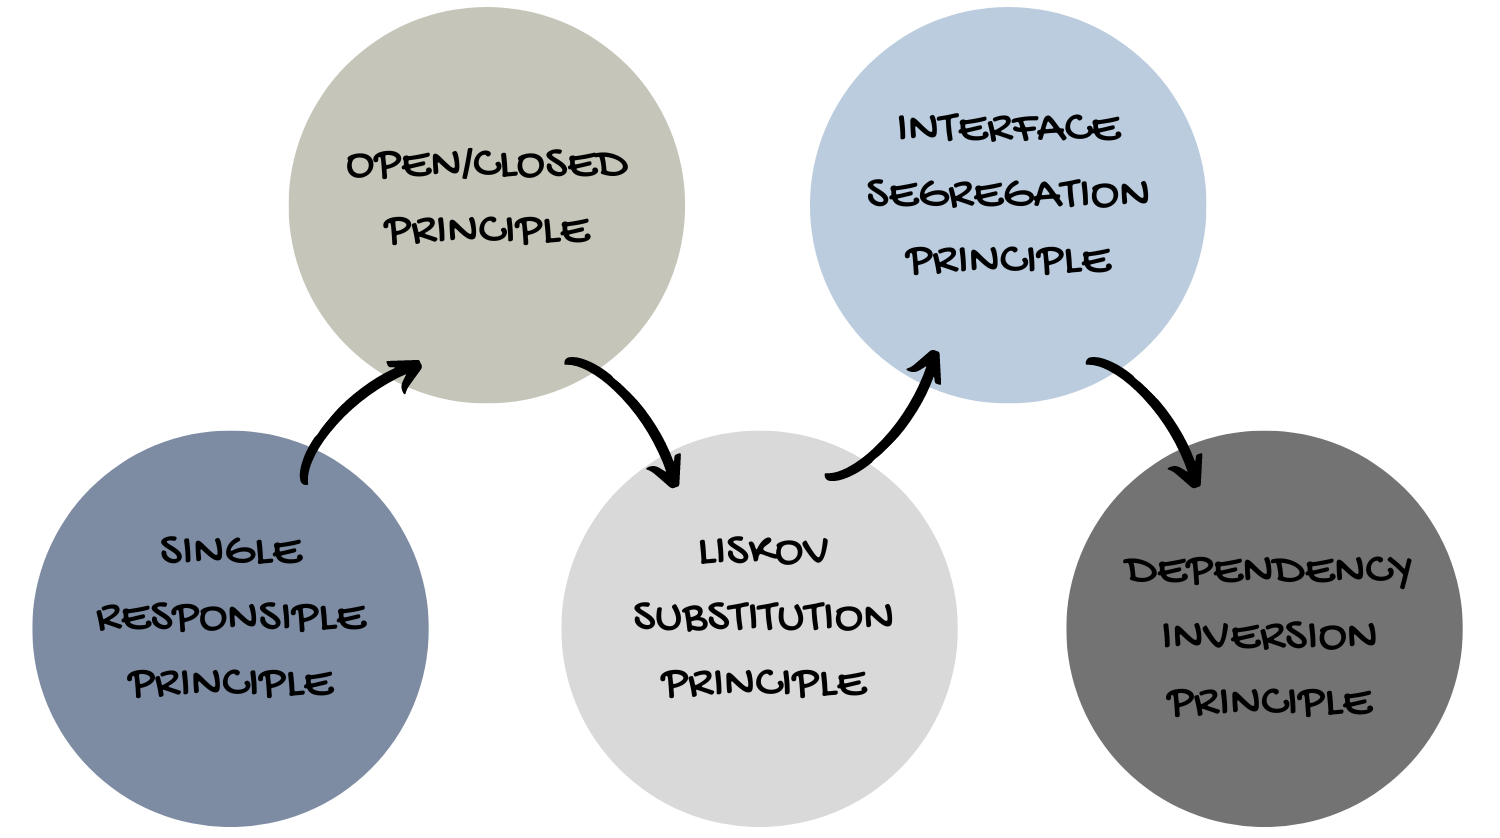
\includegraphics[scale=0.2]{solid.png}
%	\caption[SOLID]{SOLID Principles}
%\end{figure}
%\section{Symptom and Disease APIs}

\section{Application Programming Interfaces}
The aim of this work is the conception and implementation of the described system. In order to achieve this goal, the application must access a database that is filled with suitable data. The information from an existing application programming interface (API) is used here, since there are no medically trained project participants who could contribute their specialized expertise to the database. The final data structure of the database is also influenced by the selection of the API. For this purpose, the two most suitable APIs are considered and their suitability for the project is determined
\subsection{NHS Health A to Z API}
The NHS, or National Health Service, is the publicly funded healthcare system of the United Kingdom. It was established in 1948 and provides a wide range of medical services to the population of the UK, including general practitioners (GPs), hospitals, and community health services. The NHS websites provides many different APIs, free for use [NHS website]. The NHS Health A to Z API is the first API that will be considered to generate data for the database.
The API offers medical information about various diseases, their symptoms, and available treatments. A user account that is provided with a subscription key must be created in order to receive data from this API. The next step is to make an HTTP call to https://api.nhs.uk/conditions. An example of a possible request in the programming language Python looks like this:
\begin{lstlisting}[language=Python, caption={Example Python Request for the Health A to Z API}]
urlDiseases = "https://api.nhs.uk/conditions/acne"
header = {
	"subscription-key" : "YOUR_SUBSCRIPTION_KEY"
}
responseDiseases = requests.request("GET", urlDiseases, headers=header)
responseData = responseDiseases.json()
\end{lstlisting}
If the request was successfull and the response contains the data in JSON format. Listing 2.3 shows a sample abbreviated response from the API.
\begin{lstlisting}[caption={Example Response for the Health A to Z API}]
{
	"@context":"http://schema.org",
	"@type":"MedicalWebPage",
	"name":"Acne",
	"copyrightHolder":{...},
	"license":"https://developer.api.nhs.uk/terms",
	"author":{...},
	"about":{...},
	"description":"...",
	"url":"https://api.nhs.uk/conditions/acne/",
	"genre":[...],
	"keywords":[...],
	"lastReviewed":[...],
	"breadcrumb":{...},
	"dateModified":"2022-05-30T14:30:18+00:00",
	"hasPart":[...],
	"relatedLink":[...],
	"contentSubTypes":[...],
	"mainEntityOfPage":[...],
	"alternativeHeadline":"Overview"
}
\end{lstlisting}
An entire text document with the server's response to the request made in listing 2.2 can be viewed by scanning the QR code shown in the appendix x.x. A positive aspect of this API is that all data is described in great detail and a large amount of knowledge can be obtained in a single query. However, it must also be mentioned that the extent of the server response just mentioned entails the difficulty of storing the data accordingly in a separate database. For example, symptoms are supplied for a disease, but only in string format as a complete sentence. This means that a symptom is described in different ways in several diseases. In order to automatically scrape this data, one would have to recognize all variations in the description of a symptom. With the amount of data that the Health A to Z API brings with it, this is almost impossible. Another limitation is that a maximum of 6 requests can be made to the interface per minute, which proves to be a serious problem in terms of runtime.

\subsection{ApiMedic Symptom Checker API}
The ApiMedic API is the second interface to be considered. ApiMedic is powered by priaid, a company that focuses on bringing together medicine, IT and business administration. Thanks to their highly specialized team composition, they offer expertise in all of the areas mentioned. The API can be addressed in two different ways:
\begin{itemize}
	\item \textbf{Sandbox API Account:}
	It is possible to get an unlimited amount of data via the sandbox account. However, the data supplied is only dummy data.
	\item \textbf{Live Basic API Account:}
	The live account allows to get the actual medical data of the API. However, there is a limitation with regard to the possible calls: ApiMedic only allows 100 calls per month to be made without charging money, further requests cost money.
\end{itemize}
Although the data that can be received from this API is not as detailed as that of the NHS API, using the data to create a data structure is simpler. It is possible to acquire diseases, bodily components, and symptoms as well as proposed symptoms and symptoms based on each body part. The following code example shows an request, made with the live account, to retrieve all diseases followed by the response of the API.
\begin{lstlisting}[language=Python, caption={Example Python Request for the ApiMedic API (all issues)}]
stringURLIssues = "https://healthservice.priaid.ch/issues?token=YOUR_TOKEN"
responseIssues = requests.request("GET", stringURLIssues)
dataIssues = responseIssues.json()
\end{lstlisting}

\begin{lstlisting}[language=Python, caption={Response for the ApiMedic API (all issues)}]
[
	{
		"ID": 130,
		"Name": "Abdominal hernia"	
	},
	{
		"ID": 170,
		"Name": "Abortion"	
	},
	{
		"ID": 456,
		"Name": "Abscess of the tonsils"	
	},
...
\end{lstlisting}
It is now possible to execute an API request that returns detailed information about each disease, using the provided IDs. Listing 2.7 shows a sample shortened response from the ApiMedic API.
\begin{lstlisting}[language=Python, caption={Example Python Request for the ApiMedic API (single issue)}]
	stringURLIssue = "https://healthservice.priaid.ch/issues/105/info?token=YOUR_TOKEN"
	responseIssue = requests.request("GET", stringURLIssue)
	dataIssue = responseIssue.json()
\end{lstlisting}

\begin{lstlisting}[language=Python, caption={Response for the ApiMedic API (single issue)}]
{
	"Description": "Measles is caused by a virus a...",
	"DescriptionShort": "Measles, also known as morbilli, ...",
	"MedicalCondition": "The infection begins with flu-like symptoms ( ...",
	"Name": "Measles",
	"PossibleSymptoms": "Burning eyes,Burning in the throat,Cough,...",
	"ProfName": "Morbilli",
	"Synonyms": "Red measles",
	"TreatmentDescription": "To prevent measles, an effort to vaccinate ..."
}
\end{lstlisting}
\noindent 
The value of the "PossibleSymptoms"-key returns an enumaration of all the symptoms of the disease. These symptoms are listed using the values of the "Name"-key for the respective symptom when querying all symptoms. This makes it easier to scrape the data accordingly and store it in a database.

\subsection{API Solution}
The question that now arises is which of the two interfaces to choose. Both APIs have advantages and disadvantages. While the NHS API provides very detailed results, it makes it difficult to use the data for the purposes intended in this work. NHS also provides data on the causes that various symptoms and conditions can have, which can be an important factor in making a diagnosis in the form of disease detection. ApiMedic delivers the data in an optimal format to use, but far less detailed than NHS. One option that is available is, to use the symptom data provided by ApiMedic as scrape material for the symptom list in the NHS. However, after an attempt to do so, only a very small amount of symptom has been recognized. This is because the same symptom is named differently in both APIs. Generating more appropriate scrape material would require full inspection of all NHS API data, to ensure getting a decent amount of data. This is not possible within the scope of this work, but should be considered for future optimizations of the system.  In the context of the bachelor thesis, the use of the ApiMedic API is preferred from the point of view of a clean database structure.

\section{NoSQL Databases}

\subsection{Introduction to NoSQL Databases}
The generic term NoSQL describes database systems that, unlike SQL databases, are not subject to the relational database model. The abbreviation NoSQL stands for "Not only SQL". The reasons why NoSQL databases have gained interest in recent years can be explained on the basis of two aspects: In contrast to relational databases, which present their data storage in table format, NoSQL databases benefit from different database models: document-oriented, key Value, graph and column databases.[Image] This wide range of different data models gives developers the benefit of being able to choose the model that best suits their application design. The resulting result is a minimization of the code to be developed for an application. In addition, NoSQL databases allow administrators to scale their data both on one machine and on hardware clusters, so data volumes can be expanded without an expensive investment in new servers.
\begin{figure}[H]
	\centering
	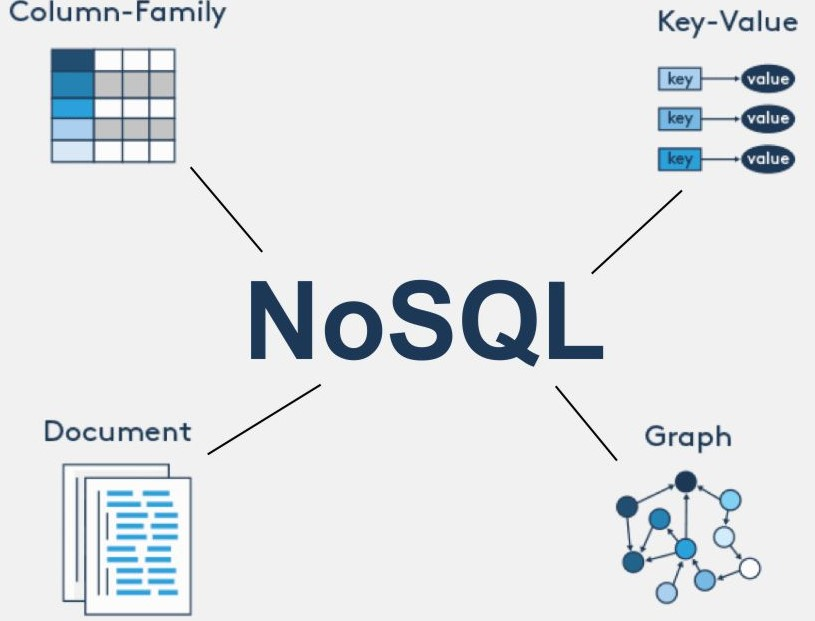
\includegraphics[scale=0.25]{nosql.jpg}
	\caption[NoSQL Data Models]{NoSQL Data Models}
\end{figure}

NoSQL databases support the use of CRUD operations.
\begin{itemize}
	\item \textbf{C:} create data
	\item \textbf{R:} read data
	\item \textbf{U:} update data
	\item \textbf{D:} delete data
\end{itemize}
The performance of some NoSQL databases even surpasses that of relational databases, especially with create and read operations. [Performance evaluation for CRUD] A detailed  performance comparison can be found in Appendix [Performance evaluation for CRUD].
\subsection{Firestore}
Cloud Firestore, more often called Google Firestore, is a cloud-hosted NoSQL database option which enables developers to store and synchronize their data in realtime, meaning that data which just got added to the database and changes made on already existing data are instantly shown to the application users. It is a part of Googles Backend-as-a-Service (BaaS) Firebase. BaaS is a concept where developers can use a platform to run their applications without managing servers and other infrastructure components. BaaS platforms offer a range of services required for applications to run, such as databases, authentication, storage and APIs. [okta.com] To use BaaS, developers must first create an account with a BaaS platform and register their application on it. The platform then provides a set of APIs and SDKs that developers can use to access the services and integrate them into their application. Most BaaS platforms offer a web-based console that developers can use to manage their applications and configure the services, so does Firebase. Since Firestore is published by Google, it comes with peak reliablitly and great performance. Something worth to mention is, that Firestore can be used with far more programming languages than Dart and is also compatible with REST and RPC APIs. [firestorewebsite] Cloud Firestore caches data that your app is actively using, so the app can write, read, listen to, and query data even if the device is offline. When the device comes back online, Cloud Firestore synchronizes any local changes back to its servers. To keep your data safe, firestore offers the opportunity to create security rules based on an individuals needs, this includes Identy and Access Management (IAM). Using firestore combined with the flutter framework one can retrieve data via the cloud\_firestore-plugin. It enables the developer to make use of the cloud firestore API. The named package also allows the developer to make use of the authentication functionality provided by the BaaS, which makes it possible for a user to register and login in an application. When trying to get data with a flutter application of a firestore database, one can simply set the GetOptions-Parameter. With defining the parameter source, one can first check, if the required data is already in the devices' cache. An example is shown in Figure 3.8.

\begin{lstlisting}[language=Python, caption={Dart - Firestore-Query}]
	
Future<DocumentSnapshot> checkCacheBeforeServer() async {
	try {
		DocumentSnapshot snapshot = await this.get(GetOptions(source: Source.cache));
		if (snapshot == null) return this.get(GetOptions(source: Source.server));
		return snapshot;
	} catch e {
		print(e);
		return this.get(GetOptions(source: Source.server));
	}
}
	
\end{lstlisting}
\noindent

\subsection{Document Databases}
There are several different NoSQL databases, which all rely on different data models. Firestore makes use of the document-based data format. This means, that data stored in the database is accessible via collections, which are filled with documents. For better understanding one can imagine a collection in Firestore as a table in relational Databases and a Document in Firestore equals a row in the relational schema. An example of that is shown in the figure x.x. Documents in Firestore store their data in a key-value-format which makes it possible for a developer to store different sort of documents in each collection. A quick view at an example makes this easier to understand: A developer wants to develop a restaurent-review application. For that he creates a collection named “restaurants” in firestore. Two of the three restaurants he now wants to add to the collection got a slogan with their brand which he wants to add to the documents, the other restaurant doesn’t have one. In a relational database he still would have to fill the “slogan” column with at least NULL-data or an empty String (or whatever datatype the column has). Firestore, or document-based databases in general, allow it, to just not add the slogan attribute to the third restaurant, which helps to only store relevant data to the database. One thing to keep in mind is, that even if the third restaurant one day gets a slogan, the developer has the possibility to add that field to the document later on. Cloud Firestore also allows it to store subcollections or complex nested objects to documents. Firestore has no option to store foreign keys in a document. The solution to create a foreign key-like mechanism is covered in the Database chapter. 

\section{Jupyter Notebook}
In order to integrate the data of the ApiMedic API into Firestore, a Python script is set up as part of this work. This is created using Jupyter Notebook and can be found in the project repository on GitHub.
  
  
\chapter{Requirements Engineering}
In order to provide a functional and relevant application, it is necessary to first determine the stakeholders who influence the project in the form of a stakeholder analysis, from which a system context can then be determined. The functional and non-functional as well as the optional requirements for the application must then be described. Based on the information gained from all of this, a domain model can then be generated, which serves as a transition to the creation of the database.

\section{Target Group and User Group}
Both senior persons and young people who, despite the difficulties mentioned in the introducition, would desire to have a diagnosis of their current health status situation are targeted by the system. One may assume that, given the age distribution of smartphone users today, the user base will be evenly split between the young and the old. In Germany, 94.2 percent of people aged 14 to 19 owned a smartphone by the year 2021, according to Statista statistics. Between the ages of 20 and 29, it is 95,5 \%, and between 30 and 39, it is 96 \%. The proportion of smartphone owners among the over 70s is still around 68 percent \cite{.smartphonenutzer}.
One more target audience are medical professionals. The application should offer an easy-to-use interface for adding and editing data in the database, eliminating the need for technical expertise. Only the doctors' attitudes about the project can provide a more specific indication of this user group's limitation. The stakeholder analysis will go into greater depth on this subject. 

\section{Stakeholder Analysis}
The first step is to identify the project's interest and demand groups. This is done through a stakeholder analysis. The societal influences on the project are looked at in the stakeholder analysis. The stakeholder analysis allows for the prediction of variables such as “power”, “interest” and potential stakeholder behavior. Stakeholders are individuals (groups), organizations, and interest groups that have the power to significantly affect a project's success. Therefore, it is essential for project managers to understand their interests and potential for influencing the project goals \cite[p. 28]{.stakeholder}. It is necessary to consider which individuals have a stake in the project's success and which individuals have the potential to influence the project in both positive and negative ways in order to identify the stakeholders. Persons affected by the project might be classified as internal or external stakeholders. 

\subsection{Internal Stakeholder}
\subsubsection{Developer}
In this project, the internal stakeholder group is relatively small. The only significant internal stakeholder will be the personification of the developer, which is also the administrator of the data bank. Due to the positive effects a successful and widely used application would have on his reputation as a developer, this person has a great, personal, interest in the project's success. The power he wields over the project is extremely high. Without him, the application development would not be possible.

\subsection{External Stakeholder}
\subsubsection{Users}
Customers, or users in the case of an application, are considered external stakeholders. They want to use a flawlessly functioning application and are keenly interested in the project's success. This can be attributed to the points mentioned in the introduction chapter. Their impact on the project appears to be significant, given that the success of an application cannot be guaranteed in the absence of a user group.
In concrete terms, the interests of the users can be written as follows:
\subsubsection{Doctors}
General practitioners and specialists make up another stakeholder group. They have the option to log in to the application and change existing database entries, as well as create new entries. Their impact on the project is moderate because the internal database manager stakeholder can expand the database without them. The power factor, however, can both rise and improve when doctors talk to their patients about the application. A doctor's negative (or positive) impression of the initiative may deter (or pique) patients, resulting in the loss (or gain) of users. As a result, individual differences in interest in the project will also exist.

\begin{figure}[h]
	\centering
	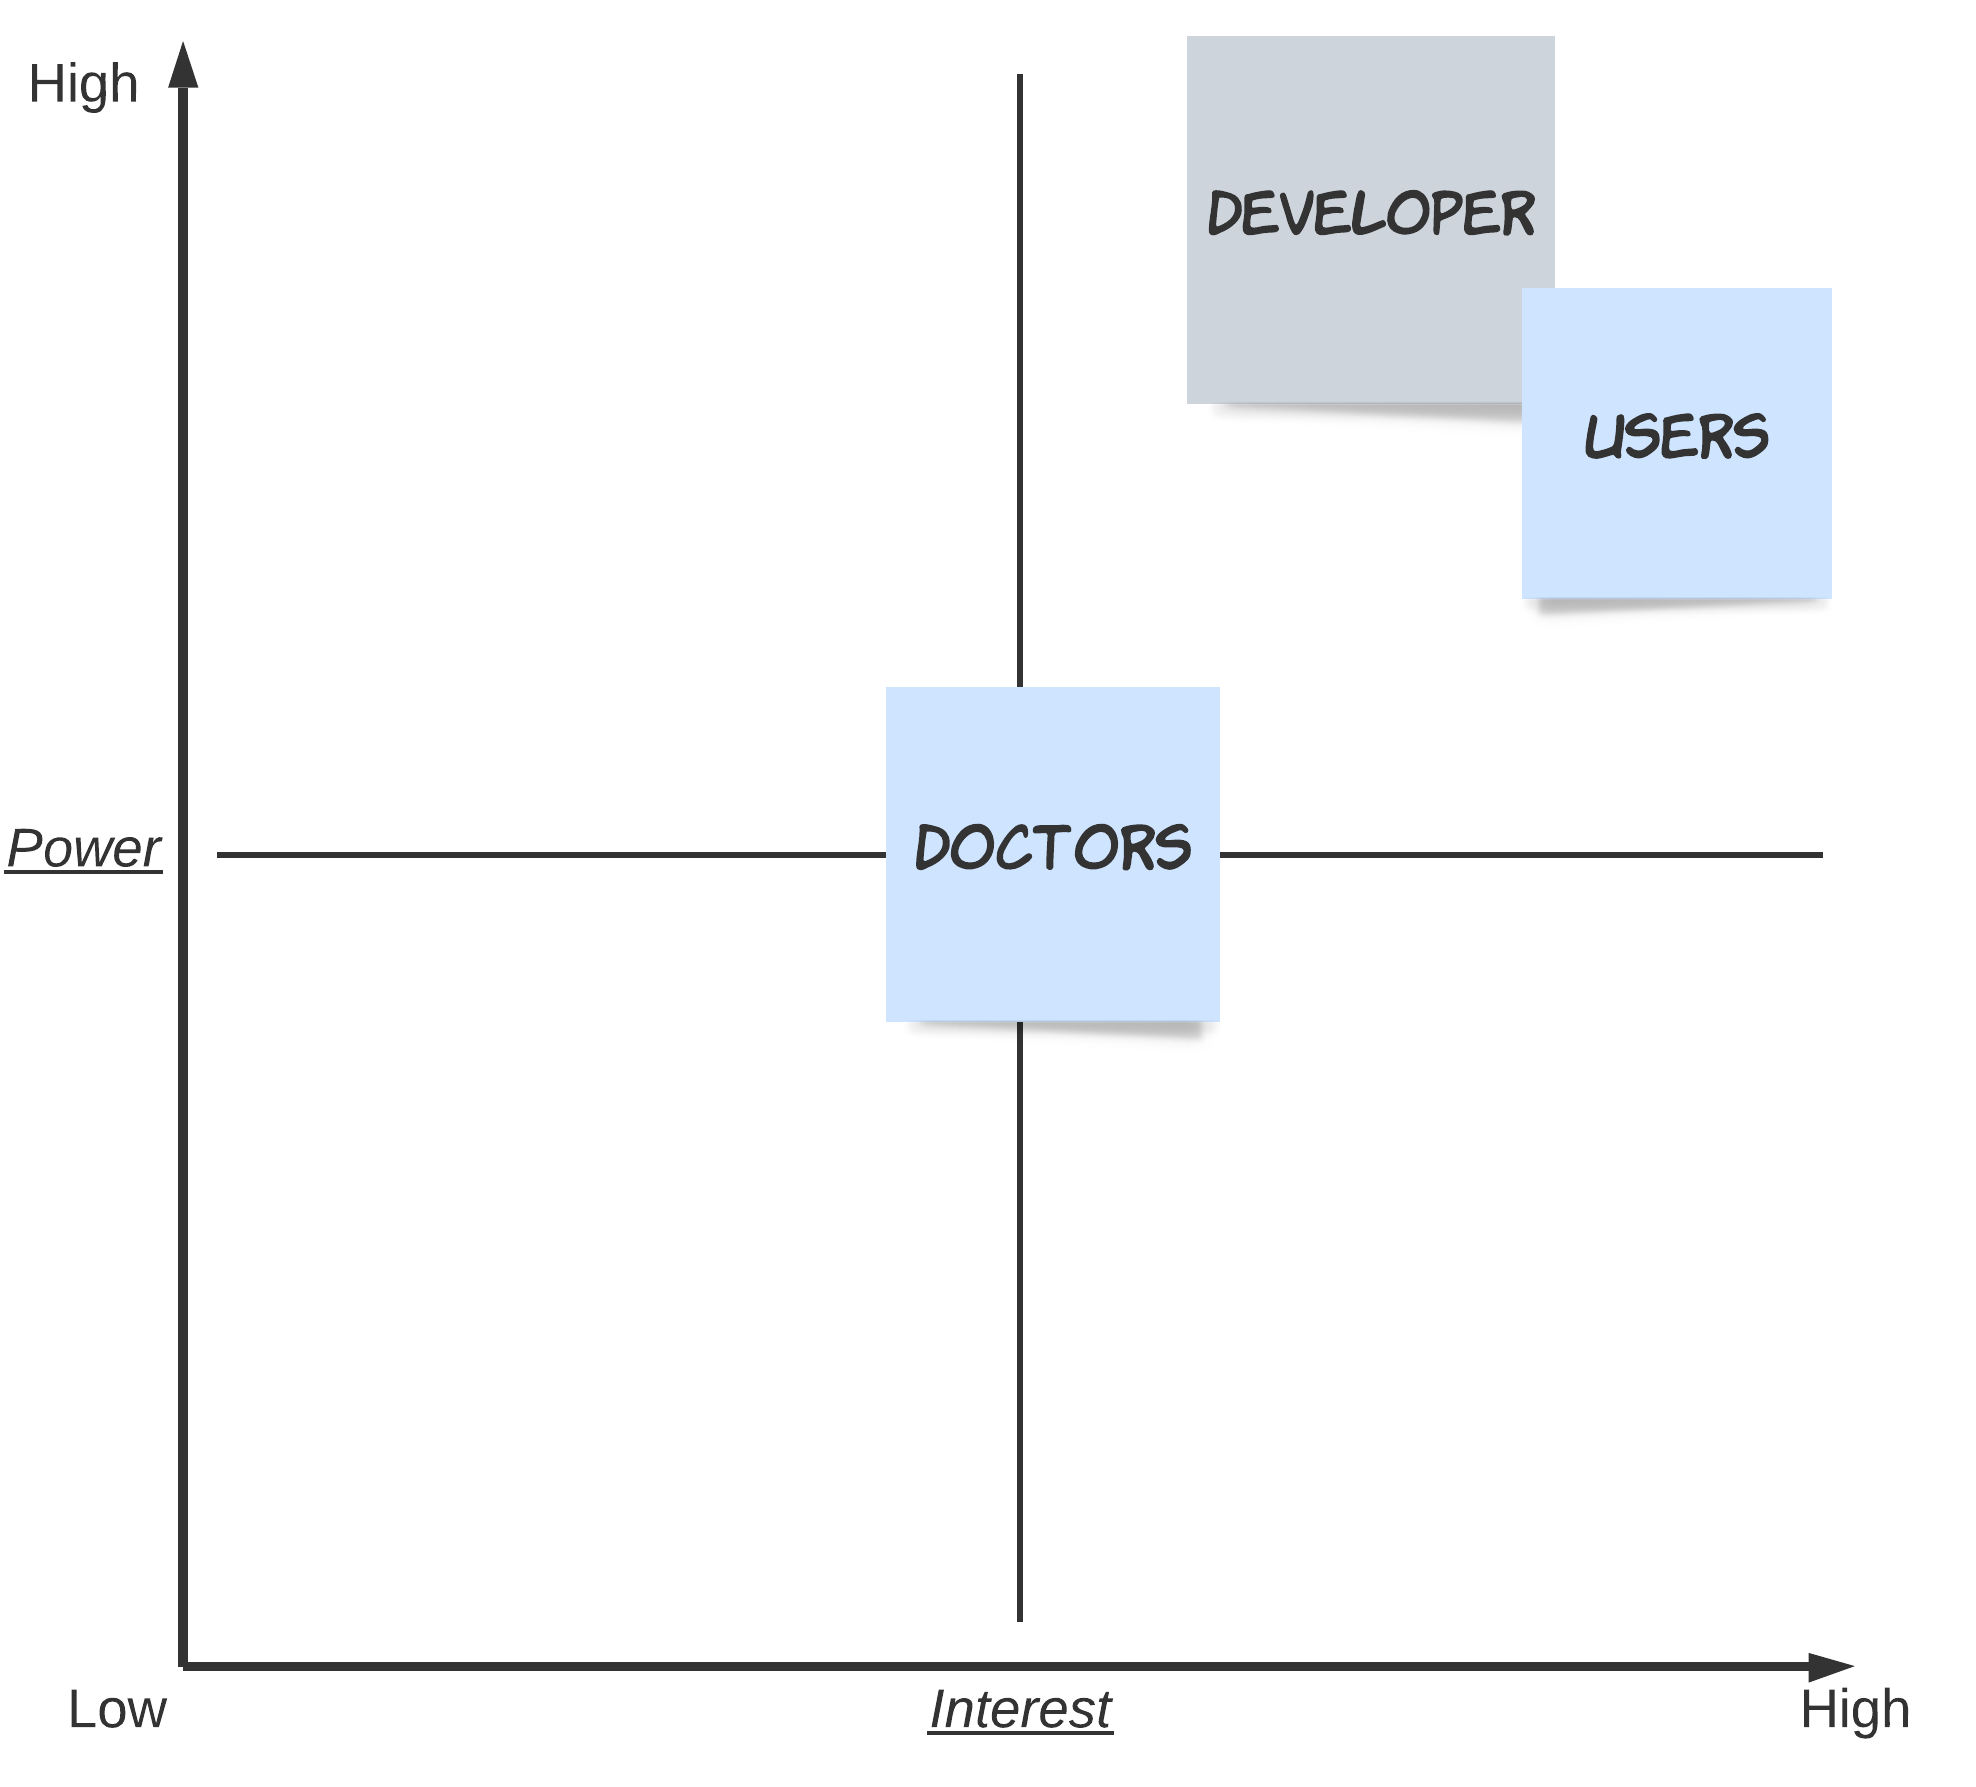
\includegraphics[scale=0.5]{stakeholder_matrix.png}
	\caption[Power/Interest Grid for Stakeholder-Analysis ]{Power/Interest Grid for Stakeholder-Analysis}
\end{figure}	

\section{System Context Diagram}
The greater environment in which a specific system or process functions is known as the system context. It covers all the outside variables and influences that affect the system's function, such as the stakeholders who are impacted by its operation, external systems, and processes with which it interacts and the policies and regulations that it must comply with. The system context can be determined using the previously performed stakeholder analysis. Determining the system context helps to get an understanding of which components interact with the system. This includes both the stakeholders and systems that influence the system.
The stakeholder groups of users and doctors can access the application via a smartphone. The developer and the database communicate with the system via direct code-based access.As already described in the APIs section, the database is filled with data from the ApiMedic API. The filling of the database will take place outside the system, in the form of a Python script (Jupyter Notebook). There surely are some aspects about privacy policy and the security of personal data of the users, especially during the verification process of the doctors. Since, in context of this bachelor thesis, the application will not be launched on the PlayStore these aspects are neglected in the system context.

\begin{figure}[h!]
	\centering
	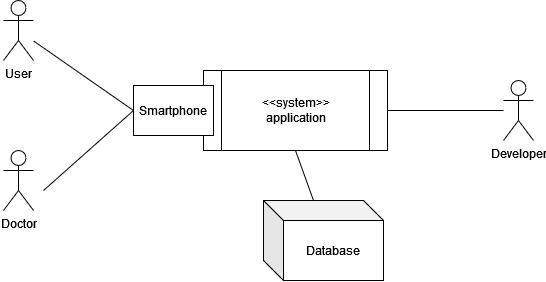
\includegraphics[scale=0.65]{system_context.png}
	\caption[System Context Diagram ]{System Context Diagram}
\end{figure}

\section{User Requirements Specification}
The requirements for an application can be divided into three categories: functional requirements, non-functional requirements and optional requirements. In this section, the different types of requirements are considered and created project-specifically.

\subsection{Optional Requirements}
As the name suggests, optional requirements of an application consist of requirements that do not necessarily have to be implemented.
\begin{table}[H]
	\begin{center}
		\scriptsize
		\def\arraystretch{2}%
		\begin{tabular}{ c|l }
			\hline
			\textbf{ID} & \textbf{Description}  \\
			\hline
			OR1 & The application should make it possible to save and download a diagnosis in PDF format  \\
			\hline
			OR2 & The application should make it possible for a user to save tips on a favorites list  \\
			\hline	
		\end{tabular}
		\normalsize
	\end{center}
	\caption{Optional Requirements}
\end{table}
\subsection{Functional Requirements}
Functional requirements are the specific capabilities, behaviors, and features that a system must have. They describe what the system must do in order to be considered successful, and provide a basis for evaluating the system's performance and functionality.
\begin{table}[H]
	\begin{center}
		\scriptsize
		\def\arraystretch{2}%
		\begin{tabular}{ c|l}
			\hline
			\textbf{ID} & \textbf{Description}  \\
			\hline
			FR1 & The application must allow the user to switch between the diagnostics and the advices view  \\
			\hline
			FR2 & The application must offer the user the option of being able to verify themselves as a doctor  \\
			\hline
			FR3 & The application must offer a doctor the opportunity to log in  \\
			\hline
			FR4 & The application must offer a doctor the opportunity to add a new record in the database  \\
			\hline
			FR5 & The application must offer a doctor the possibility of editing data records in the database  \\
			\hline
			FR6 & The application must allow a user to start a new diagnosis  \\
			\hline
			FR7 & The application must enable a user to save a diagnosis  \\
			\hline	
			FR8 & The application must enable a user to view his saved diagnoses again  \\
			\hline
			FR9& The application must allow a user to abort his diagnostic procedure at any time \\
			\hline
			FR10 & The application must allow a user to delete saved diagnoses  \\
			\hline
			FR11 & The application must allow a doctor to abort adding or editing data at any time\\
			\hline
		\end{tabular}
		\normalsize
	\end{center}
	\caption{Functional Requirements}
\end{table}

\subsection{Non-functional Requirements}
After the functional requirements have been determined, the non-functional requirements are now considered. Non-functional requirements can be described by not dealing with the direct interaction of a user with the application, but with the system-specific properties. This includes, for example, the reliability of the application, but also safety aspects. [Buch google]
\begin{table}[H]
	\begin{center}
		\scriptsize
		\def\arraystretch{2}%
		\begin{tabular}{ c|l }
			\hline
			\textbf{ID} & \textbf{Description}  \\
			\hline
			NFR1 & The application must make correct diagnoses  \\
			\hline
			NFR2 & The application must be usable for patients without registration  \\
			\hline
			NFR3 & The application should have a graphical interface that can be used intuitively  \\
			\hline	
		\end{tabular}
		\normalsize
	\end{center}
	\caption{Non-Functional Requirements}
\end{table}


\section{Use Cases}
The architectural goal of the application is to be designed to provide an optimal user experience for both, patients and doctors. In order to ensure this, it is necessary to determine, before the actual development, which use cases the software has to cover, i.e. the externally visible interactions of the users with the system. This ensures that the application meets the wishes of the users and that they actually use the application. In addition, possible ambiguities are revealed and required data structures are determined. Possible problems that may arise during use of the application are most likely to be found during the process and technical solutions can then be worked out. Experience has shown that use cases also make it easier for a developer to create the objects that have to be created with an object-oriented programming language in the early development process more precisely and to recognize and implement inheritance options at an early stage. Some use cases can be identified from the functional and optional requirements set out above. Figure 3.3 shows the resulting use case diagram, which has been shortened to the most relevant use cases. 

\begin{figure}[h]
	\centering
	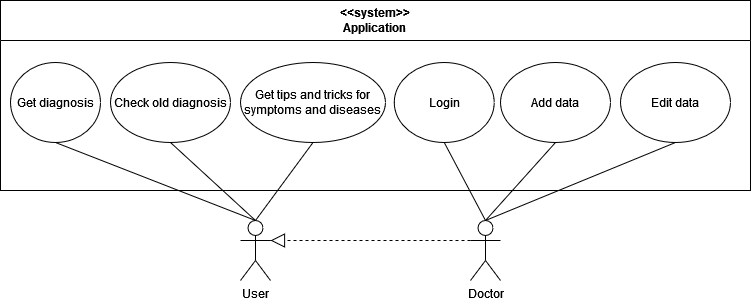
\includegraphics[scale=0.6]{use_case_diagram.png}
	\caption[Use Case Diagram]{Use Case Diagram}
\end{figure}
\noindent
The use cases are described in detail in the following sections. The resulting use case tables for each of them can be found in the appendix [].

\subsection{Get Diagnosis}
The first use case is described by the fact that a user would like to receive a diagnosis \textbf{[FR6]}. The actors who can carry out this use case are both patients, i.e. normal users, and doctors. In this application, doctors represent a subclass of users. In order to start the disease determination, the trigger, which will be implemented in the form of a button, must be pressed. The system then responds by displaying the view to enter and specify symptoms. As soon as the actor has finished specifying the symptoms, the system calculates the possible diseases and displays them to the actor in the form of a diagnosis. The actor now has the opportunity to decide whether he wants to end the use case by exiting the diagnostic view or saving the diagnosis \textbf{[FR7]}, which is indicated by pressing the save button. The system then saves the diagnosis. Optionally, the actor should also be able to save the diagnosis as a PDF on his device \textbf{[OR1]}. During the process, the user has the option to cancel the symptom statement at any time, which ends the use case by returning to the main page of the application \textbf{[FR10]}.

\subsection{Review Received Diagnoses}
After the user has received his diagnosis, he should be able to look at old diagnoses again \textbf{[FR8]}. The prerequisite for seeing such a diagnosis is that the actor has previously saved it, when the diagnosis was made. A view is provided in the application in which saved diagnoses are displayed in a list. Clicking on such a diagnosis starts the use case, whereupon the system opens the detailed view of the diagnosis. The use case is ended by clicking on the back button provided for this purpose. While the diagnosis is being viewed, the user has the option of deleting the selected diagnosis, which is triggered by clicking on the icon provided for this purpose and is answered by deleting the diagnosis from the system. In this use case, too, the user is given the opportunity to save his diagnosis as a PDF \textbf{[OR1]}, the procedure for this corresponds to that of the "Get Diagnosis" use case.

\subsection{Login}
As already mentioned in the project goal, doctors should be given the opportunity to log into the application \textbf{[FR3]}. The trigger for the use case is the click on the login button. Once the button is pressed, the application will display the login page. There, the actor has the opportunity to enter his credentials, whereupon the system checks whether these are stored in the database. Should the result be positiv, the doctor will be logged in and the system will display the doctor's dashboard. The prerequisite, for the use case to be carried out without errors, is that the doctor has been able to verify himself as such beforehand \textbf{[FR2]}. If this has not yet happened, the user has the opportunity to click on the verify button, where he will be prompted to carry out this process and will be logged in if it is successful. Should it be not successfull, because the user can not verify himself as a doctor, the system will continue showing error messages to the acteur.  If the doctor is verified, but the system cannot find the entered credentials, an error message is displayed by the application and the user, suspecting that the credentials have been entered incorrectly, is asked to check his user data and try again after making a correction.

\subsection{Add Data}
Provided that he is logged in, a doctor can now add data to the database \textbf{[FR4]}. In order to do this, he must press the button provided for this purpose. The system then displays the blank template for a data record, in which the doctor can enter the data he wants to add. As soon as he has done this and pressed the confirm button, the system adds the data record to the database and saves it in his data list as well. If the actor presses the confirm button without entering anything in each data field, the application will display an error notification on the screen, prompting the user to fill in all data fields. If the user wishes to cancel the process, he is free to press the button provided for this at any time, whereupon the system closes the view and the use case ends \textbf{[FR11]}. 

\subsection{Edit Data}
In addition to the functionality to create new datasets, the doctor should be able to expand and edit existing datasets \textbf{[FR5]}. The structure of this use case is similar to the previously described use case of adding new data. The doctor must first be in the view in which all existing data records are displayed in list format. There he has the opportunity to click on one of these data sets, which signals to the system that it must now display the editing screen for the selected data set. In this view, the doctor can now make the desired changes and press the confirm button. The application will then update the record in the database and the use case will be terminated. As before when adding new data records, the doctor has the option to end the process at any time \textbf{[FR11]}.

\subsection{Get Tips and Tricks for Symptoms and Diseases}
The final use case worth mentioning is viewing advice on illnesses \textbf{[FR1]}. A user has the option to go to the view for all advice that Doctors have uploaded. Once he's navigated there and the system shows the predicted view, he can click on one of the pieces of advice there and it will be shown to him in detail. Optionally, the user can save the advice as a favorite by clicking on the button provided for this purpose \textbf{[OR2]}. 

\section{Domain Model}
Domain modeling is a major modeling topic in Agile development at scale because there is frequently a gap between comprehending the issue domain and the interpretation of requirements. It depicts the solution as a collection of domain objects that collaborate to satisfy system-level scenarios. [internetseite SAFe] The quintessence of the object-oriented analysis step is the decomposition of a domain into problem-relevant concepts or objects. A domain model is a visual representation of the problem-relevant domain classes of a domain. With the help of UML notation, a domain model is represented by a set of class diagrams in which no operations are defined, it presents a conceptual perspective and can show domain objects or classes, as well as associations between domain classes and attributes of domain classes. [UML 2 Buch]  Domain modeling is a major modeling topic in Agile development at scale because there is frequently a gap between comprehending the issue domain and the interpretation of requirements. Identifying domain entities and their connections, derived from a grasp of system-level requirements, offers a good foundation for understanding and supports practitioners in designing systems for maintainability, testability, and incremental development. [internetseite SAFe] Finding conceptual classes by recognizing substantive phrases is an effective technique to domain modeling. [Buch UML2]

\begin{itemize}
	\item A person is a \textbf{user} of the application.
	\item A \textbf{user} chooses a \textbf{body part}.
	\begin{itemize}
		\item A \textbf{body part} can be associated with different \textbf{symptoms}.
		\item A \textbf{user} selects a \textbf{symptom} and specifies the selected symptom by narrowing down (selecting) \textbf{proposed symptoms}, the \textbf{time of occurrence} and the \textbf{symptom intensity}. The information obtained is summarized as a textbf{user-specified symptom}.
	\end{itemize}
	\item One or more \textbf{user-specified symptoms} lead to the calculation of one or more possible \textbf{diseases}.
	\begin{itemize}
		\item A \textbf{disease} has different \textbf{symptoms}.
	\end{itemize}
	\item A \textbf{diagnosis} consists of one or more \textbf{diseases}.
	\item \textbf{Doctors} are special \textbf{users} of the application.
	\item \textbf{Doctors} can add/edit \textbf{advices}, \textbf{symptoms}, \textbf{body parts} and \textbf{diseases}.
	\item \textbf{Users} can view \textbf{advices}.  
\end{itemize}
\noindent
The information just obtained makes it easier to create the domain model. The entities user, symptom, user-specified symptom, body part, diseases, doctor, advice and diagnosis can already be recognized. Based on that information a domain model can be created. 
\begin{figure}[H]
	\centering
	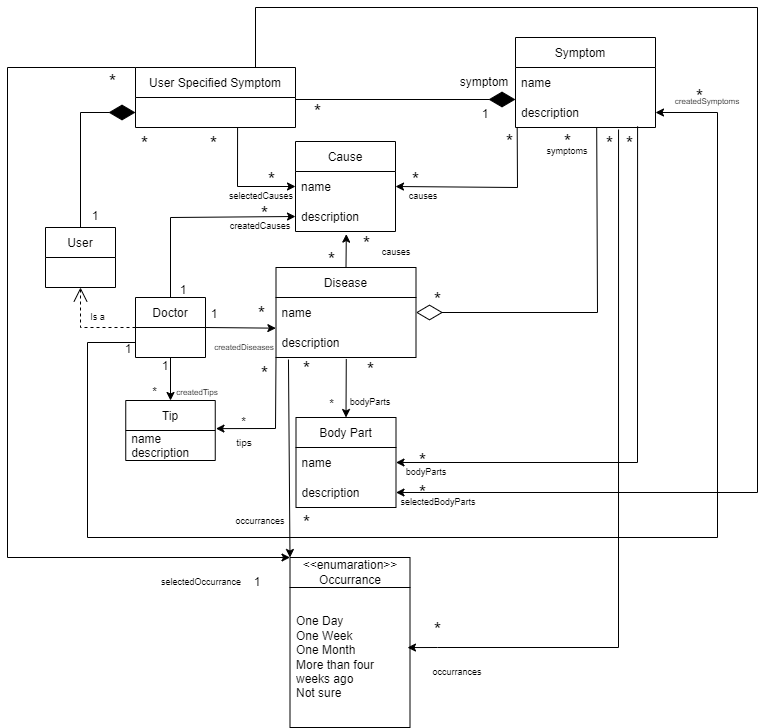
\includegraphics[scale=0.2]{domain_model.png}
	\caption[Domain Model]{Domain Model}
\end{figure}
\noindent
Based on the domain model and the previously obtained information, the database development can now be started. Later on, the chapter optimizations also addresses some aspects that have been neglected at the moment.

 
  
  
\chapter{The Database}
The following chapter is devoted to creating the Firestore database for the application. For this purpose, the JSON data records provided by the ApiMedic API are examined more closely in order to be able to design a database structure. After the successful data conception, the data sets are integrated into Firestore via a Python script. This procedure is also documented using a notebook (Jupyter Notebook) and is described there in more detail.

\section{Data Structure}
The data structure of the database is based on the decision that the ApiMedic API will be the main supplier of the data. The basic data structure can already be guessed from the domain model, which is shown in Figure 4.4. Firestore supports the following datatypes: String, Number, Boolean, Map, Array, Null, Timestamp, Geopoint and Reference. With a closer look at the API's JSON responses, the data structures can be formed.

\subsection{Examination of the JSON-Structure of ApiMedic}
ApiMedic does not provide any actual documentation. Instead, they give interested users the opportunity to test the HTTP requests directly via the ApiMedic website. To access the API, a HTTP request must be sent. The URL of the endpoint, the HTTP method and, if necessary, other parameters and headers must be specified. All inquiries can be made via a request to the following URL: \textbf{https://healthservice.priaid.ch/} in connection with the corresponding path to the desired file resource. The API responses can then be extracted from the HTTP message body in the form of a JSON object.

\subsubsection{Body Part}
\begin{itemize}
	\item \textbf{Get all Body Regions:  /body/locations?token=\{your\_token\}}
	\newline
	If the request is successful (status code 200), all body regions that are stored in the API form the output.
		\begin{center}
			\begin{tabular}{ | c| c| c | } 
  				\hline
  				Name of Field& Content & Datatype \\ 
  				\hline
  				ID & ID of the body region & Integer \\ 
  				\hline
 				Name & Name of the body region & String \\ 
  				\hline
			\end{tabular}
		\end{center}
With the help of the ID of the body regions, the individual body parts of a region can be determined.
	\item \textbf{Get all Body Parts:  /body/locations/\{body\_region\_id\}?token=\{your\_token\}}
	\newline
If the request is successful (status code 200), all body locations that are stored in the API form the output.
		\begin{center}
			\begin{tabular}{ | c| c| c | } 
  				\hline
  				Name of Field& Content & Datatype \\ 
  				\hline
  				ID & ID of the body location & Integer \\ 
  				\hline
 				Name & Name of the body location & String \\ 
  				\hline
			\end{tabular}
		\end{center}
	\item \textbf{Get all Body Parts:  /body/locations/\{body\_region\_id\}/\{gender\_id\}?token=\{your\_token\}}
	\newline
If the request is successful, all body locations that are stored in the API form the output. The IDs of the genders are values ranging from 0 to 3. 
		\begin{center}
		\scriptsize
			\begin{tabular}{ | c| c| c | } 
  				\hline
  				Name of Field& Content & Datatype \\ 
  				\hline
  				ID & ID of the symptom & Integer \\ 
  				\hline
 				Name & Name of the symptom & String \\ 
  				\hline
  				HasRedFlag & Indicates whether the symptom has been classified as critical & Boolean \\ 
  				\hline
  				HealthSymptomLocationIDs & IDs of the body locations that are affected by this symptom & Array[Integer] \\ 
  				\hline
 				ProfName & Professional name of the symtom & String \\
				\hline 			
 				Synonyms & Synonyms of the symptom & Array[String] \\
 				\hline
			\end{tabular}
		\normalsize
		\end{center}

\end{itemize}
Instead of storing all body areas, all explicit body parts and their possible symptoms will be stored in Firestore. Based on the information obtained from successful HTTP requests, the Firestore structure can be defined as shown below.
\newline
\textbf{Collection: body\_parts}
		\begin{center}
			\begin{tabular}{ | c| c| c | } 
  				\hline
  				Name of Document-field& Content & Datatype \\ 
  				\hline
  				name & Name of the body part & String \\ 
  				\hline
 				symptoms & List of all symptom ids of the body part  & Array[String] \\ 
  				\hline
			\end{tabular}
		\end{center}
The ids of the documents are formed from the name of the respective object. Here, spaces are simply replaced by a "\_" and the name string is stripped of leading and trailing spaces using the Python function .strip(). The id generation method should never be used for real world applications. However, it simplifies the legibility in the context of this bachelor thesis. Firestore saves all the data in form of documents which can be created using .doc(\{document\_id\}).set(\{...\}).  When performing this operation, the document is automatically assigned the specified ID, making it unnecessary to store the id in the document itself.

\subsubsection{Ressource Symptom}
\begin{itemize}
		\item \textbf{Get all Symptoms :  /symptoms?token=\{your\_token\}}
\newline		
If the request is successful, all symptoms that are stored in the API form the output.
		\begin{center}
			\begin{tabular}{ | c| c| c | } 
  				\hline
  				Name of Field& Content & Datatype \\ 
  				\hline
  				ID & ID of the symptom & Integer \\ 
  				\hline
 				Name & Name of the symptom & String \\ 
  				\hline
			\end{tabular}
		\end{center}

\item \textbf{Get all proposed Symptoms:  /symptoms/proposed?symptoms=[\{symptom\_ids\}]\newline\&gender=\{gender\_name\}\&year\_of\_birth=\{birthyear\_YYYY\}?token=\{your\_token\}}
\newline
Unlike the query regarding all symptoms of a body part, the values of the genders are not to be given as an ID, but in the form of full names, i. e. "male" and "female".
	\begin{center}
			\begin{tabular}{ | c| c| c | } 
  				\hline
  				Name of Field& Content & Datatype \\ 
  				\hline
  				ID & ID of the proposed symptom & Integer \\ 
  				\hline
 				Name & Name of the proposed symptom & String \\ 
  				\hline
			\end{tabular}
		\end{center}
\end{itemize}
Since all ids of the symptoms for each body part are already stored in each body part document, there is no need to add the body part ids to the symptom anymore. Because of that, all that is needed to be stored is the name of the symptom and the ids of the proposed symptoms.
\newline
\textbf{Collection: symptoms}
		\begin{center}
			\begin{tabular}{ | c| c| c | } 
  				\hline
  				Name of Document-field& Content & Datatype \\ 
  				\hline
  				name & Name of the body part & String \\ 
  				\hline
 				proposed\_symptoms & List of all proposed symptoms ids of the symptom  & Array[String] \\ 
  				\hline
			\end{tabular}
		\end{center}
\subsubsection{Ressource Disease}
\begin{itemize}
	\item \textbf{Get all issues (diseases):  /issues?token=\{your\_token\}}
	\newline
	If the request is successful (status code 200), all diseases that are stored in the API form the output.
		\begin{center}
			\begin{tabular}{ | c| c| c | } 
  				\hline
  				Name of Field& Content & Datatype \\ 
  				\hline
  				ID & ID of the body region & Integer \\ 
  				\hline
 				Name & Name of the body region & String \\ 
  				\hline
			\end{tabular}
		\end{center}
With the help of the ID of the body regions, the individual disease can be determined.
	\item \textbf{Get a single issue:  /issues/\{issue\_id\}?token=\{your\_token\}}
	\newline
If the request is successful (status code 200), the requested issue forms the output.
		\begin{center}
			\begin{tabular}{ | c| c| c | } 
  				\hline
  				Name of Field& Content & Datatype \\ 
  				\hline
  				Description & Description of the disease & String \\ 
  				\hline
 				DescriptionShort & Short description of the disease & String \\ 
  				\hline
  				MedicalCondition & Description of the symptoms & String \\ 
  				\hline
  				Name & Name of the disease & String \\ 
  				\hline
  				PossibleSymptoms & All symptoms of the disease, comma separated string & String \\ 
  				\hline
  				ProfName & Professional name of the disease & String \\ 
  				\hline
  				Synonyms & Synonyms of the disease & String \\ 
  				\hline
  				Treatment & Treatment steps for the disease & String \\
  				\hline 
			\end{tabular}
		\end{center}
\end{itemize}
The resources provided by the issues are stored in the Firestore database under the diseases collection. For the purposes of the work, only the name, description, symptoms and treatment recommendation are extracted and stored.
\newline
\textbf{Collection: diseases}
		\begin{center}
			\begin{tabular}{ | c| c| c | } 
  				\hline
  				Name of Document-field& Content & Datatype \\ 
  				\hline
  				name & Name of the body part & String \\ 
  				\hline
 				description & List of all symptom ids & Array[String] \\ 
  				\hline
  				treatment & Treatment recomendation of the disease & String \\ 
  				\hline
			\end{tabular}
		\end{center}
\subsubsection{Advice}
The advice generated by doctors is not part of the ApiMedic API data resources. They are created directly by users (doctors) of the application and require a title, description, associated symptoms and associated diseases. Taken together, this results in the document structure shown in Table x.x.
\textbf{Collection: advices}
		\begin{center}
			\begin{tabular}{ | c| c| c | } 
  				\hline
  				Name of Document-field& Content & Datatype \\ 
  				\hline
  				name & Title of the advice& String \\ 
  				\hline
 				description & Description of the advice & String \\ 
  				\hline
  				symptoms & List of associated symptom ids & Array[String]\\ 
  				\hline
  				diseases & List of associated disease ids & Array[String]\\ 
  				\hline
			\end{tabular}
		\end{center}
\subsubsection{Doctor}
Doctors have the opportunity to register with the database. To do this they will be asked to enter an email and a password. Firestore allows all of this to happen without involving a dedicated collection of users. Nevertheless, it makes sense to do this, since user data could possibly be expanded at a later date. An example of this is that records added by a doctor should also be referenced in his account. This requires a collection that stores the user data of the respective doctor in separate documents. The user ID is automatically generated by Firestore in the form of a hash value during registration.
\textbf{Collection: doctors}
		\begin{center}
			\begin{tabular}{ | c| c| c | } 
  				\hline
  				Name of Document-field& Content & Datatype \\  
  				\hline
  				email & E-Mail-Adress of the doctor & String \\
  				\hline
			\end{tabular}
		\end{center}
\subsubsection{User, User Specified Symptom, Diagnose, SymptomIntensity and NovelityFactor}
The user-defined symptoms are not stored in the database, but are only generated temporarily and locally in the system during the diagnosis. The reason for not saving the user-specific symptoms is that a user does not have to log in to the application and therefore no user document is created in the database through which the symptoms could be traced back to the user. Only the individual attributes of the object are stored in the diagnosis in order to be able to understand the diagnosis when it is called up again. The classes users and diagnoses, as well as the enumerations symptoms intensity and novelty factor will not be stored in the database, but will be, too, modeled internally in the system. There, the diagnoses are to be stored locally on the smartphone, which ensures that no personal data of the user is stored in the database.

\section{Inserting the Data into the Database}
Adding the records to the database requires a few steps, which have been summarized with the help of Jupyter Notebook. The notebook can be downloaded by following the link of the QR code in the appendix x.

\section{Connecting the Database with the Flutter Project}
After the successful data generation, the database can now be integrated into the application. For this, the scheme provided by the Flutter developers is followed.
\begin{itemize}
	\item Importing the required package \textbf{cloud\_firestore} to the flutter application
	\item 
\end{itemize}
  
  
%% PLANUNG %% 

\chapter{Conception and Design}
This section deals with the conception of the graphical user interface and the implementation options of the application.
\section{Graphical User Interface}
First, a look is taken at whether the graphical user interface plays an important role in applications at all. For this purpose, a question on this topic was also included in the survey already mentioned. The answers on this question revealed that the graphical interface of an application, in fact, plays a role in terms of the trustworthiness of the application. Figure 6.1 shows the results of the survey-question.
\begin{figure}[H]
	\centering
	\includegraphics[scale=0.4]{appUiImportant.png}
	\caption[Survey Question]{Survey Question - Trustworthiness of the Application based on the UI}
\end{figure}
\noindent
Respondents of the survey were also given the opportunity to choose between three different UIs. The graphical interface should be adapted to the choice made by the people interviewed.
\subsection{Conceptual Design of the Graphical User Interface}
The UI can be designed based on the requirements analysis of the application and the information obtained from it. As already defined there, the application should be designed to be as intuitive and easy to use as possible. The implementation of the design of the user interface, for the android version, is based on suggestions from the material.io website [material.io], an open-source design system developed by google. The integration of the design components into the Flutter application is simplified thanks to the pre-installed material.dart package. This package is based on the source mentioned and currently supports version 2 of material.io. Support for the current version 3 of Material Design is still being worked on.
\noindent
One goal of this application is to be designed to be intuitive. In his book "UI is COMMUNICATION", Everett N. McKay described an intuitive UI as follows: 
\begin{quote}
	\textit{"A UI is intuitive when target users understand its behavior and effect without use of reason, memorization, experimentation, assitance, or training."} - Everett N McKay [Quelle]
\end{quote}
In order to meet this definition, goals that the user interface should meet could be set before the graphic user interface is designed.\\
\noindent
On the one hand, the user should be able to recognize immediately that a component of the screen is a widget that he can operate. The system must then show the user that something has been triggered by his action. This can be done, for example, through feedback in the form of a loading circle if required data still needs to be loaded, or in the form of a new screen, pop-up or similar design components. [everett] Another step that can be taken to make the application more intuitive is the correct (short) labeling of the respective components. For example, a corresponding text, or even better imagery [ess mobile interac design cameron, seite 172], should be stored on a confirmation button. In addition, it should be ensured that surface components do not change their positions. This ensures that users can rely on their previous interactions and thus learn how to use the application. Minimalism is becoming a trend not only in the real world, but also in the digital world. This can also be seen looking at the most popular graphical interface of the survey, shown in Figure 6.2. The associated surfaces can be found in Appendix x.
\begin{figure}[H]
	\centering
	
\includegraphics[scale=0.4]{whichUI.png}
	\caption[Survey Question]{Survey Question - Which UI}
\end{figure}
\noindent
Designing the application as minimalistic as possible has the advantage that the graphical interface is not overloaded and thus the user is not overwhelmed by different widgets at all. This may make it easier for the user to better interpret the use of specific elements. Another factor that plays a role in user-friendliness is to use familiar design patterns. This ensures that users are already familiar with the handling of the app elements and that there is no confusion regarding the use. 

\subsection{Description of the Views and Thoughts on the Implementation in Flutter}
This section presents the individual views that are made available to users. In addition, first thoughts on possible implementation ways for those views, working with Flutter, are considered.
\subsubsection{\textbf{Home Screen}}
The first view that a user will encounter when installing or opening the application is the home screen. There, he should be given the opportunity to switch between the different views that are necessary for his use: diagnosis creation, diagnosis overview and advice view. In addition, every user should be able to access the login screen for doctors, since they can verify themselves there as such. The navigation to create a diagnosis is implemented in the form of a button and labeled with a corresponding, clearly formulated text. To get to all other screens, a list view of all options is offered, in which there are various clickable fields that trigger navigation to the corresponding screen when clicked. In Flutter, this view can be achieved through several different components. The most important widgets can be used in the form of children in a column. In order to implement the clickable forwarding elements to other views, one should use a ListView, storing children of the widget GestureDetector, which allows any widget to be clickable. The childrens can be stored in an external modifiable list, this allows you to simplify the integration of new categories at a later point in time. A mock-up of a possible home screen can be found in Appendix x.

\subsubsection{\textbf{View for the diagnostic process}}
The screen to start a diagnosis should be designed as simple as possible. Users can adress on which body part they are feeling their symptoms. Based on their selection the application shows all symptoms associated with the body part, which then can be selected and afterwards specified by the user. The widget \textit{Stepper} is a possible implementation option. It gives the developer the opportunity to easily implement a type of step-by-step tool. For this purpose, only all steps for generating a diagnosis are created and filled with the appropriate data. The full code for an example Stepper-widget can be found in the appendix x.

%	\scriptsize
%	\begin{lstlisting}[caption=Stepper for Body Part Selection]
%		...
%		  List<String> selectedBodyParts = [];
%		...
%		Stepper(
%		type: stepperType,
%		physics: ScrollPhysics(),
%		currentStep: _currentStep,
%		onStepTapped: (step) => tapped(step),
%		steps: [
%			...,
%			Step(
%				title: const Text('Location of the Symptoms'),
%				subtitle: const Text(
%				"Please select the body Part ...",),
%				title: const Text("Body Parts"),
%				onTap: (values) {
%					setState(() {
%						selectedBodyParts = values;
%					});},),
%			isActive: _currentStep >= 0,
%			state:
%			_currentStep >= 0 ? StepState.complete : StepState.disabled,
%			),
%			...
%	\end{lstlisting}
%	\normalsize
\subsubsection{\textbf{Login Screen (Doctor)}}
The login screen is displayed to the user immediately after clicking on the navigation tool labeled "Doctor Panel". There he will be offered the option to log in or register. This is achieved by simply adding editable textfields for the needed user input: email, password and confirmation password. If the user has already created a user account in a previous session, has verified himself as a medical profressional and has then been logged in, he will be forwarded to the actual doctor panel without any further need to log in. An exception is given if he has previously logged out. With the help of the flutter\_login package, a developer can implement the login process in Dart very easily. Appendix x demonstrates the use of the FlutterLogin-plugin. There are also options to customize the appeareance of the login-form.
%\scriptsize
%\begin{lstlisting}[caption=Stepper for Body Part Selection]
%	...
%	FlutterLogin(
%		logo: const AssetImage('assets/images/login.png'),
%		title: 'Please login to continue',
%		onLogin: AuthService.instance.signIn,
%		onSignup: AuthService.instance.registration,
%		onConfirmRecover: AuthService.instance.resetPassword,
%		onSubmitAnimationCompleted: (() {
%			Navigator.of(context).pop();
%			AppNavigator.push(Routes.doctorPanel);}),
%		onRecoverPassword: (_) => Future(() => null),)
%	...
%\end{lstlisting}
%\normalsize
\subsubsection{\textbf{Screen with all body parts, diseases, advices and symptoms (Doctor)}}
The doctor panel should contain all the necessary data related to the records stored in the database. Here, a doctor can switch between the different collections. A good implementation method for this would be the BottomNavigationBar. It contains various navigation elements, which all change to their data view when you click on them. The data views show a list of the data stored in the associated Firestore collection. Care should be taken to ensure that it is recognizable that you can click on the list elements. When the user clicks on such an element, the system redirects to the edit view for the associated record. In order to be able to store new data quickly, a FloatingActionButton can also be integrated, which opens a small menu by clicking on it, where all the data add options for the doctor are listed. Clicking on a listing item then opens the associated add view.
\subsubsection{\textbf{View for adding and editing data (Doctor)}}
In order to make the views as intuitive as possible, it is advisable to make the graphical interface as uncluttered as possible. Furthermore, here only text fields are included for the data records where possible. For the selection of related data for a data set (e.g. symptoms for an illness), a button is placed on the view which, when clicked, generates and displays a dialog with the content of all symptoms in the database. Ideally, this dialog should also contain a search bar so that the user is not forced to scroll through the large number of data records. Both, the edit view and the view to add new records, consist of a form widget. In this it is possible to transfer text fields as children, which can be modified by a user. The distinction here is only between the initial value of the text fields. While the data stored in the database for the associated data record is displayed in the edit view, when a new data tuple is created, only an empty text field with a note regarding the data field is specified.
\subsubsection{\textbf{View with all saved diagnoses}}
The diagnoses view is represented by a vertical list of all diagnoses. A ListView is used here. This ListView contains all diagnostic data that the user has previously saved on his device. Clicking on a diagnosis element in the list opens the detailed view of this diagnosis. It shows the date on which the diagnosis was made, which symptoms the user specified and which illnesses resulted from the calculation of the probability of diseases. This are represented in the form of a bar chart. At the end of the diagnosis, the diseases are listed again in list form, together with their description and treatment recommendations.

\subsubsection{\textbf{View with all advices stored in the database (User) }}
The recommendation screen is laid out similarly to the diagnosis screen. Here, too, the data from Firestore is displayed in the form of a vertical list and a click opens the detailed description of the advice. This detailed view simply consists of text fields which contain the data from the document fields.
\subsection{Mock-ups and Survey regarding the Trustworthiness of Mock-up Designs}
With the description of the screens and the first development approaches, mock-ups could already be created with the help of Canva. These can be found in Appendix x. As parat of a survey, it was founrd out whether the basic idea of the graphic design would speak for trustworthiness and whether the participants woudl have inutitively known how to interact with the interface. The results are presented below.

%\section{The Symptom Graph}
%\subsection{Performance Evaluation}
%\subsection{Scalability Comparison}

\chapter{Implementation}
Based on the specifications from the previous chapter, it is now possible to open the app to implement. This chapter describes the technologies used for the development of this application. The project structure is also examined in more detail.
\section{Project Structure}
When developing software systems in the client-server, it is advised to make sure that the project and class structures are divided into three different layers.
\begin{itemize}
	\item \textbf{Data Layer}
	\newline
	The data layer takes care of retrieving the (raw) data from the database. For this purpose, a class named DatabaseService is generated as part of the Flutter application, which can be instantiated.
	\scriptsize
		\begin{lstlisting}[caption=Stepper for Body Part Selection]
		class DatabaseService {
			/* CREATE AN INSTANCE OF THE DATABASE */
			DatabaseService._();
			static DatabaseService _instance = DatabaseService._();
			static DatabaseService get instance => _instance;
		}
		\end{lstlisting}
	\normalsize
	Using DatabaseService.instance.\_methodName, each method of the service can now be called globally from anywhere in the project.
	\item \textbf{Business Logic Layer}
	\newline
	With the help of the business layer, the data that is now received from the database service can be converted into models with which the system can work accordingly. For this purpose, a ConvertService can be created similar to Listing 7.1, which can be instantiated in the same way. This now queries the data using the DatabaseService.instance and converts the data which is supplied by the Firestore API in the form of DocumentSnapshots, Streams or QuerySnapshots. The data models for this are presented in the Data Models section.
	\item \textbf{Presentation Layer}
	\newline
	This layer takes care of mapping the data to the graphical interface. To do this, it queries the model data of the ConvertService and creates the widgets that are to be displayed accordingly.
\end{itemize}
In project development, it is increasingly interesting how applications receive their data. As part of this work, this will happen through API queries to the Firestore database. The whole procedure is also known as the client-server model. An example of the communication process, together with the services that just got described, is shown in Figure 7.1. 
\begin{figure}[H]
	\centering
	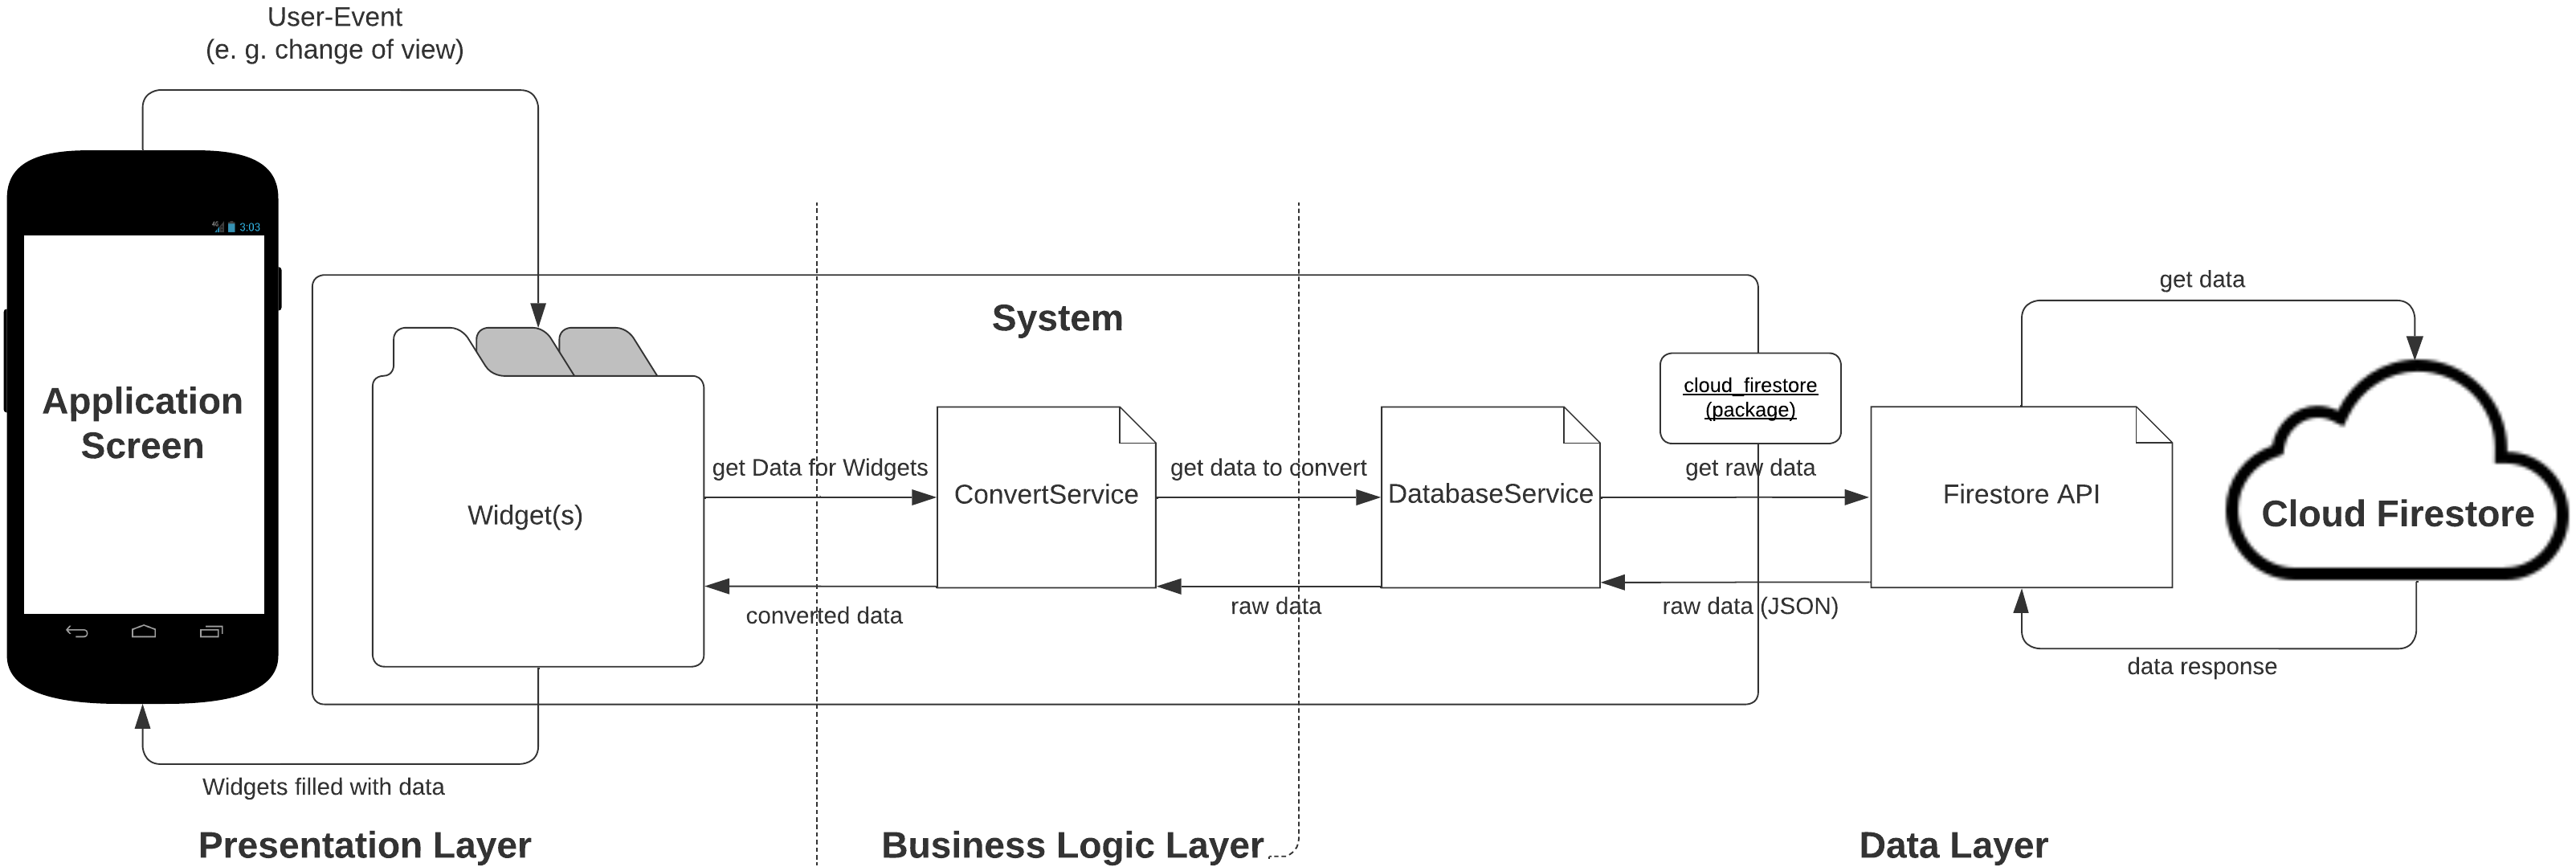
\includegraphics[scale=0.2]{api_flow.png}
	\caption[Client-Server Request Flow]{Client-Server Request Flow}
\end{figure}
\noindent
\subsection{Routing in the Application}
Another step that can be taken to keep the project structure as clean as possible is to lay out the navigation in an extra class. In this work, a class that is named AppNavigator is created for this purpose. This navigator can then be called globally using a defined method AppNavigator.push(Route pRoute). The route parameter is an element of an enumeration which refers to different views of the application. All AppNavigator code can be found in Appendix x.
\section{Data Models}
The data model into which the ConvertService converts the raw data of the DataService is based on the document structure stored in the database. When scraping the data of the JSON responses, the data is converted as follows: String$\,\to\,$String, Array$\,\to\,$List, Map<key, value>$\,\to\,$Map<String, dynamic>, Number$\,\to\,$num. Listing 7.2 shows the resulting model for symptoms. All other Models can be found in the appendix x.
\scriptsize
\begin{lstlisting}[caption=Model for Symptoms]
class Symptom {
	final String? id;
	String name;
	List<String> symptoms;
	
	Symptom({this.id, required this.name, required this.symptoms});
	
	Map<String, dynamic> toMap() {
		return {
			'name': name,
			'proposed_symptoms': List<String>.from(
			symptoms.map((x) => x),
			),};}
	
	Symptom.fromDocumentSnapshot(DocumentSnapshot<Map<String, dynamic>> doc)
		: id = doc.id,
		name = doc.data()!["name"],
		symptoms = List<String>.from(
		doc.data()!["proposed_symptoms"].toList(),);	
}
\end{lstlisting}
\normalsize


\section{Algorithms for the Attribution of Symptoms to potential Diseases}
\subsection{Solution based on the Naive Bayes Algorithm}
\subsubsection{Weighting of the Symptoms within the Application}
\subsection{K-nearest Neighbors Algorithm}
\subsection{Beyesian Networks}
\section{Evaluation of the Algorithms}
\section{Diagnoses}
\subsection{Generate Diagnose PDF}
\subsection{Store PDF Locally on Device}

  
  
%% PROOF OF CONCEPT %% 





  
  
%% FAZIT %% 

\chapter{General Overview of the Application}
\section{Testing the Application}
\section{Survey: Would Respondents use this Application and put their trust in it}


  
  \include{kapitel/60_fazit}
  
  \include{kapitel/70_fazit}
  \printbibliography %Citavi 5
  
\end{document}